All of {\ttfamily oomph-\/lib\textquotesingle{}s} existing elements implement the {\ttfamily Generalised\+Element\+::output}(...) functions, allowing the computed solution to be documented via a simple call to the {\ttfamily Mesh\+::output}(...) function, e.\+g.


\begin{DoxyCode}
\textcolor{comment}{// Open output file}
ofstream output\_file(\textcolor{stringliteral}{"output.dat"})

\textcolor{comment}{// Call the mesh's output function which loops over the }
\textcolor{comment}{// element and calls theirs...}
Problem::mesh\_pt()->output(output\_file);
\end{DoxyCode}


By default, the output is written in a format that is suitable for displaying the data with \href{http://www.tecplot.com}{\tt tecplot,} a powerful and easy-\/to-\/use commercial plotting package -- possibly a somewhat odd choice for a an open-\/source library.

We also provide the capability to output data in a format that is suitable for display with \href{http://www.paraview.org}{\tt paraview}, an open-\/source 3D plotting package. For elements for which the relevant output functions are implemented (they are defined as broken virtual functions in the {\ttfamily Finite\+Element} base class) output files for all the elements in a certain mesh (here the one pointed t by {\ttfamily Bulk\+\_\+mesh\+\_\+pt}) can be written as

 
\begin{DoxyCodeInclude}
 \textcolor{comment}{// Output solution to file in paraview format}
 some\_file.open(filename);
 Bulk\_mesh\_pt->output\_paraview(some\_file,npts);
 some\_file.close();

\end{DoxyCodeInclude}


where the unsigned integer {\ttfamily npts} controls the number of plot points per element (just as in the tecplot-\/based output functions). If {\ttfamily npts} is set to 2, the solution is output at the elements\textquotesingle{} vertices. For larger values of {\ttfamily npts} the solution is sampled at greater number of (equally spaced) plot points within the element -- this makes sense for higher-\/order elements, i.\+e. elements in which the finite-\/element solution is not interpolated linearly between the vertex nodes. It is important to note that when displaying such a solution in paraview\textquotesingle{}s \char`\"{}\+Surface with Edges\char`\"{} mode, the \char`\"{}mesh\char`\"{} that is displayed does not represent the actual finite element mesh but is a finer auxiliary mesh that is created merely to establish the connectivity between the plot points.

Paraview makes it possible to animate sequences of plots from time-\/dependent simulations. To correctly animate results from temporally adaptive simulations (where the timestep varies) paraview can operate on pvd files which provide a list of filenames and the associated time. These can be written automatically from within {\ttfamily oomph-\/lib}, using the functions in the {\ttfamily Paraview\+Helper} namespace\+:

 
\begin{DoxyCodeInclude}
\textcolor{comment}{//=================paraview\_helper=================================}
\textcolor{comment}{/// Namespace for paraview-style output helper functions }
\textcolor{comment}{}\textcolor{comment}{//=================================================================}
\textcolor{keyword}{namespace }ParaviewHelper
\{
\textcolor{comment}{}
\textcolor{comment}{ /// Write the pvd file header}
\textcolor{comment}{} \textcolor{keyword}{extern} \textcolor{keywordtype}{void} write\_pvd\_header(std::ofstream &pvd\_file);
 \textcolor{comment}{}
\textcolor{comment}{ /// \(\backslash\)short Add name of output file and associated continuous time}
\textcolor{comment}{ /// to pvd file.}
\textcolor{comment}{} \textcolor{keyword}{extern} \textcolor{keywordtype}{void} write\_pvd\_information(std::ofstream &pvd\_file,
                                   \textcolor{keyword}{const} std::string& output\_filename,
                                   \textcolor{keyword}{const} \textcolor{keywordtype}{double}& time);
 \textcolor{comment}{}
\textcolor{comment}{ /// Write the pvd file footer}
\textcolor{comment}{} \textcolor{keyword}{extern} \textcolor{keywordtype}{void} write\_pvd\_footer(std::ofstream &pvd\_file);

\}

\end{DoxyCodeInclude}


Once the pvd file is opened, call {\ttfamily Paraview\+Helper\+::write\+\_\+pvd\+\_\+header}(...) to write the header information required by paraview; then add the name of each output file and the value of the associated value of the continuous time, using {\ttfamily Paraview\+Helper\+::write\+\_\+pvd\+\_\+information}(...). When the simulation is complete write the footer information using {\ttfamily Paraview\+Helper\+::write\+\_\+pvd\+\_\+footer}(...), then close to the pvd file.

Currently, the paraview output functions are only implemented for a relatively small number of elements but it is straightforward to implement them for others.

The \href{../../FAQ/html/index.html}{\tt F\+AQ} contain an entry that discusses how to display {\ttfamily oomph-\/lib\textquotesingle{}s} output with \href{http://www.gnuplot.info}{\tt gnuplot} and \href{../../FAQ/html/index.html#tecplot}{\tt how to adjust {\ttfamily oomph-\/lib\textquotesingle{}s} output functions to different formats.}

Angelo Simone has written a python script that converts {\ttfamily oomph-\/lib\textquotesingle{}s} output to the vtu format that can be read by \href{http://www.paraview.org}{\tt paraview}. This has since been improved and extended significantly with input from Alexandre Raczynski and Jeremy van Chu. The conversion script can currently deal with output from meshes that are composed of 2D triangles and quad and 3D brick and tet elements.

The {\ttfamily oomph-\/lib} distribution contains three scripts\+:


\begin{DoxyItemize}
\item \href{../../../bin/oomph-convert.py}{\tt {\ttfamily bin/oomph-\/convert.\+py }\+:} The python conversion script itself. ~\newline
~\newline

\item \href{../../../bin/oomph-convert}{\tt {\ttfamily bin/oomph-\/convert }\+:} A shell script wrapper that allows the processing of multiple files. ~\newline
~\newline

\item \href{../../../bin/makePvd}{\tt {\ttfamily bin/make\+Pvd}\+:} A shell script the creates the {\ttfamily $\ast$} {\ttfamily }.pvd files required by paraview to produce animations.
\end{DoxyItemize}

 

\hypertarget{index_py}{}\section{The oomph-\/convert.\+py script for single files}\label{index_py}
\hypertarget{index_py_sample}{}\subsection{An example session}\label{index_py_sample}

\begin{DoxyEnumerate}
\item Add {\ttfamily oomph-\/lib\textquotesingle{}s} bin directory to your path (in the example shown here, {\ttfamily oomph-\/lib} is installed in the directory {\ttfamily /home/mheil/version185/oomph})\+: ~\newline
~\newline

\begin{DoxyCode}
biowulf: 10:31:50$ PATH=$PATH:/home/mheil/version185/oomph/bin
\end{DoxyCode}
 ~\newline

\item Here is what\textquotesingle{}s in the current directory at the moment\+: {\ttfamily curved\+\_\+pipe.\+dat} is the {\ttfamily oomph-\/lib} output produced from \href{../../navier_stokes/curved_pipe/html/index.html}{\tt a simulation of steady flow through a curved pipe.} ~\newline
~\newline

\begin{DoxyCode}
biowulf: 11:05:10$ ll
total 824
-rw-r--r--    1 mheil    users        2292 May 21 09:19 curved\_pipe.dat
\end{DoxyCode}
 ~\newline

\item Run {\ttfamily oomph-\/convert.\+py} ~\newline
~\newline

\begin{DoxyCode}
biowulf: 11:16:18$  oomph-convert curved\_pipe.dat

-- Processing curved\_pipe.dat
  oomph-convert.py, ver. 20110531
Convert from oomph-lib Tecplot format to VTK XML format.
Dimension of the problem: 3
Plot cells defined
Field variables =  4
Conversion started
Coordinate defined
Connectivities defined
Offset defined
Element types defined
Field data defined
Conversion done
  Output file name: curved\_pipe.vtu
\end{DoxyCode}
 ~\newline

\item We now have the corresponding {\ttfamily $\ast$} {\ttfamily }.vtu file ~\newline
~\newline

\begin{DoxyCode}
biowulf: 11:32:08$ ll
total 1024
-rw-r--r--    1 mheil    users      329874 Jun 21 09:19 curved\_pipe.dat
-rw-r--r--    1 mheil    users      705294 Jun 21 11:16 curved\_pipe.vtu
\end{DoxyCode}
 ~\newline

\item ...which we can visualise with paraview\+: ~\newline
~\newline

\begin{DoxyCode}
biowulf: 11:34:08$ paraview --data=curved\_pipe.vtu
\end{DoxyCode}

\end{DoxyEnumerate}



 



If your output file is invalid or contains elements that cannot currently be converted, you can use the {\ttfamily -\/p} option (followed by 2 or 3 to indicate the spatial dimension of the problem) to extract points only\+:


\begin{DoxyCode}
biowulf: 11:16:13$ oomph-convert.py -p2 soln0.dat
\end{DoxyCode}
 ~\newline
 The output is now a .vtp data file (Visualization Toolkit Polygonal) which is also supported by Paraview. To display your .vtp data, use the  
\begin{DoxyImageNoCaption}
  \mbox{
\includegraphics[width=0.03\textwidth]{glyph_button}}
\end{DoxyImageNoCaption}
 {\ttfamily Glyph} filter (displaying the points as crosses, say). Here is a representative plot in which \href{../../poisson/fish_poisson/html/index.html}{\tt the adaptive solution of a 2D Poisson equation in a fish-\/shaped domain} is displayed with points.

 
\begin{DoxyImageNoCaption}
  \mbox{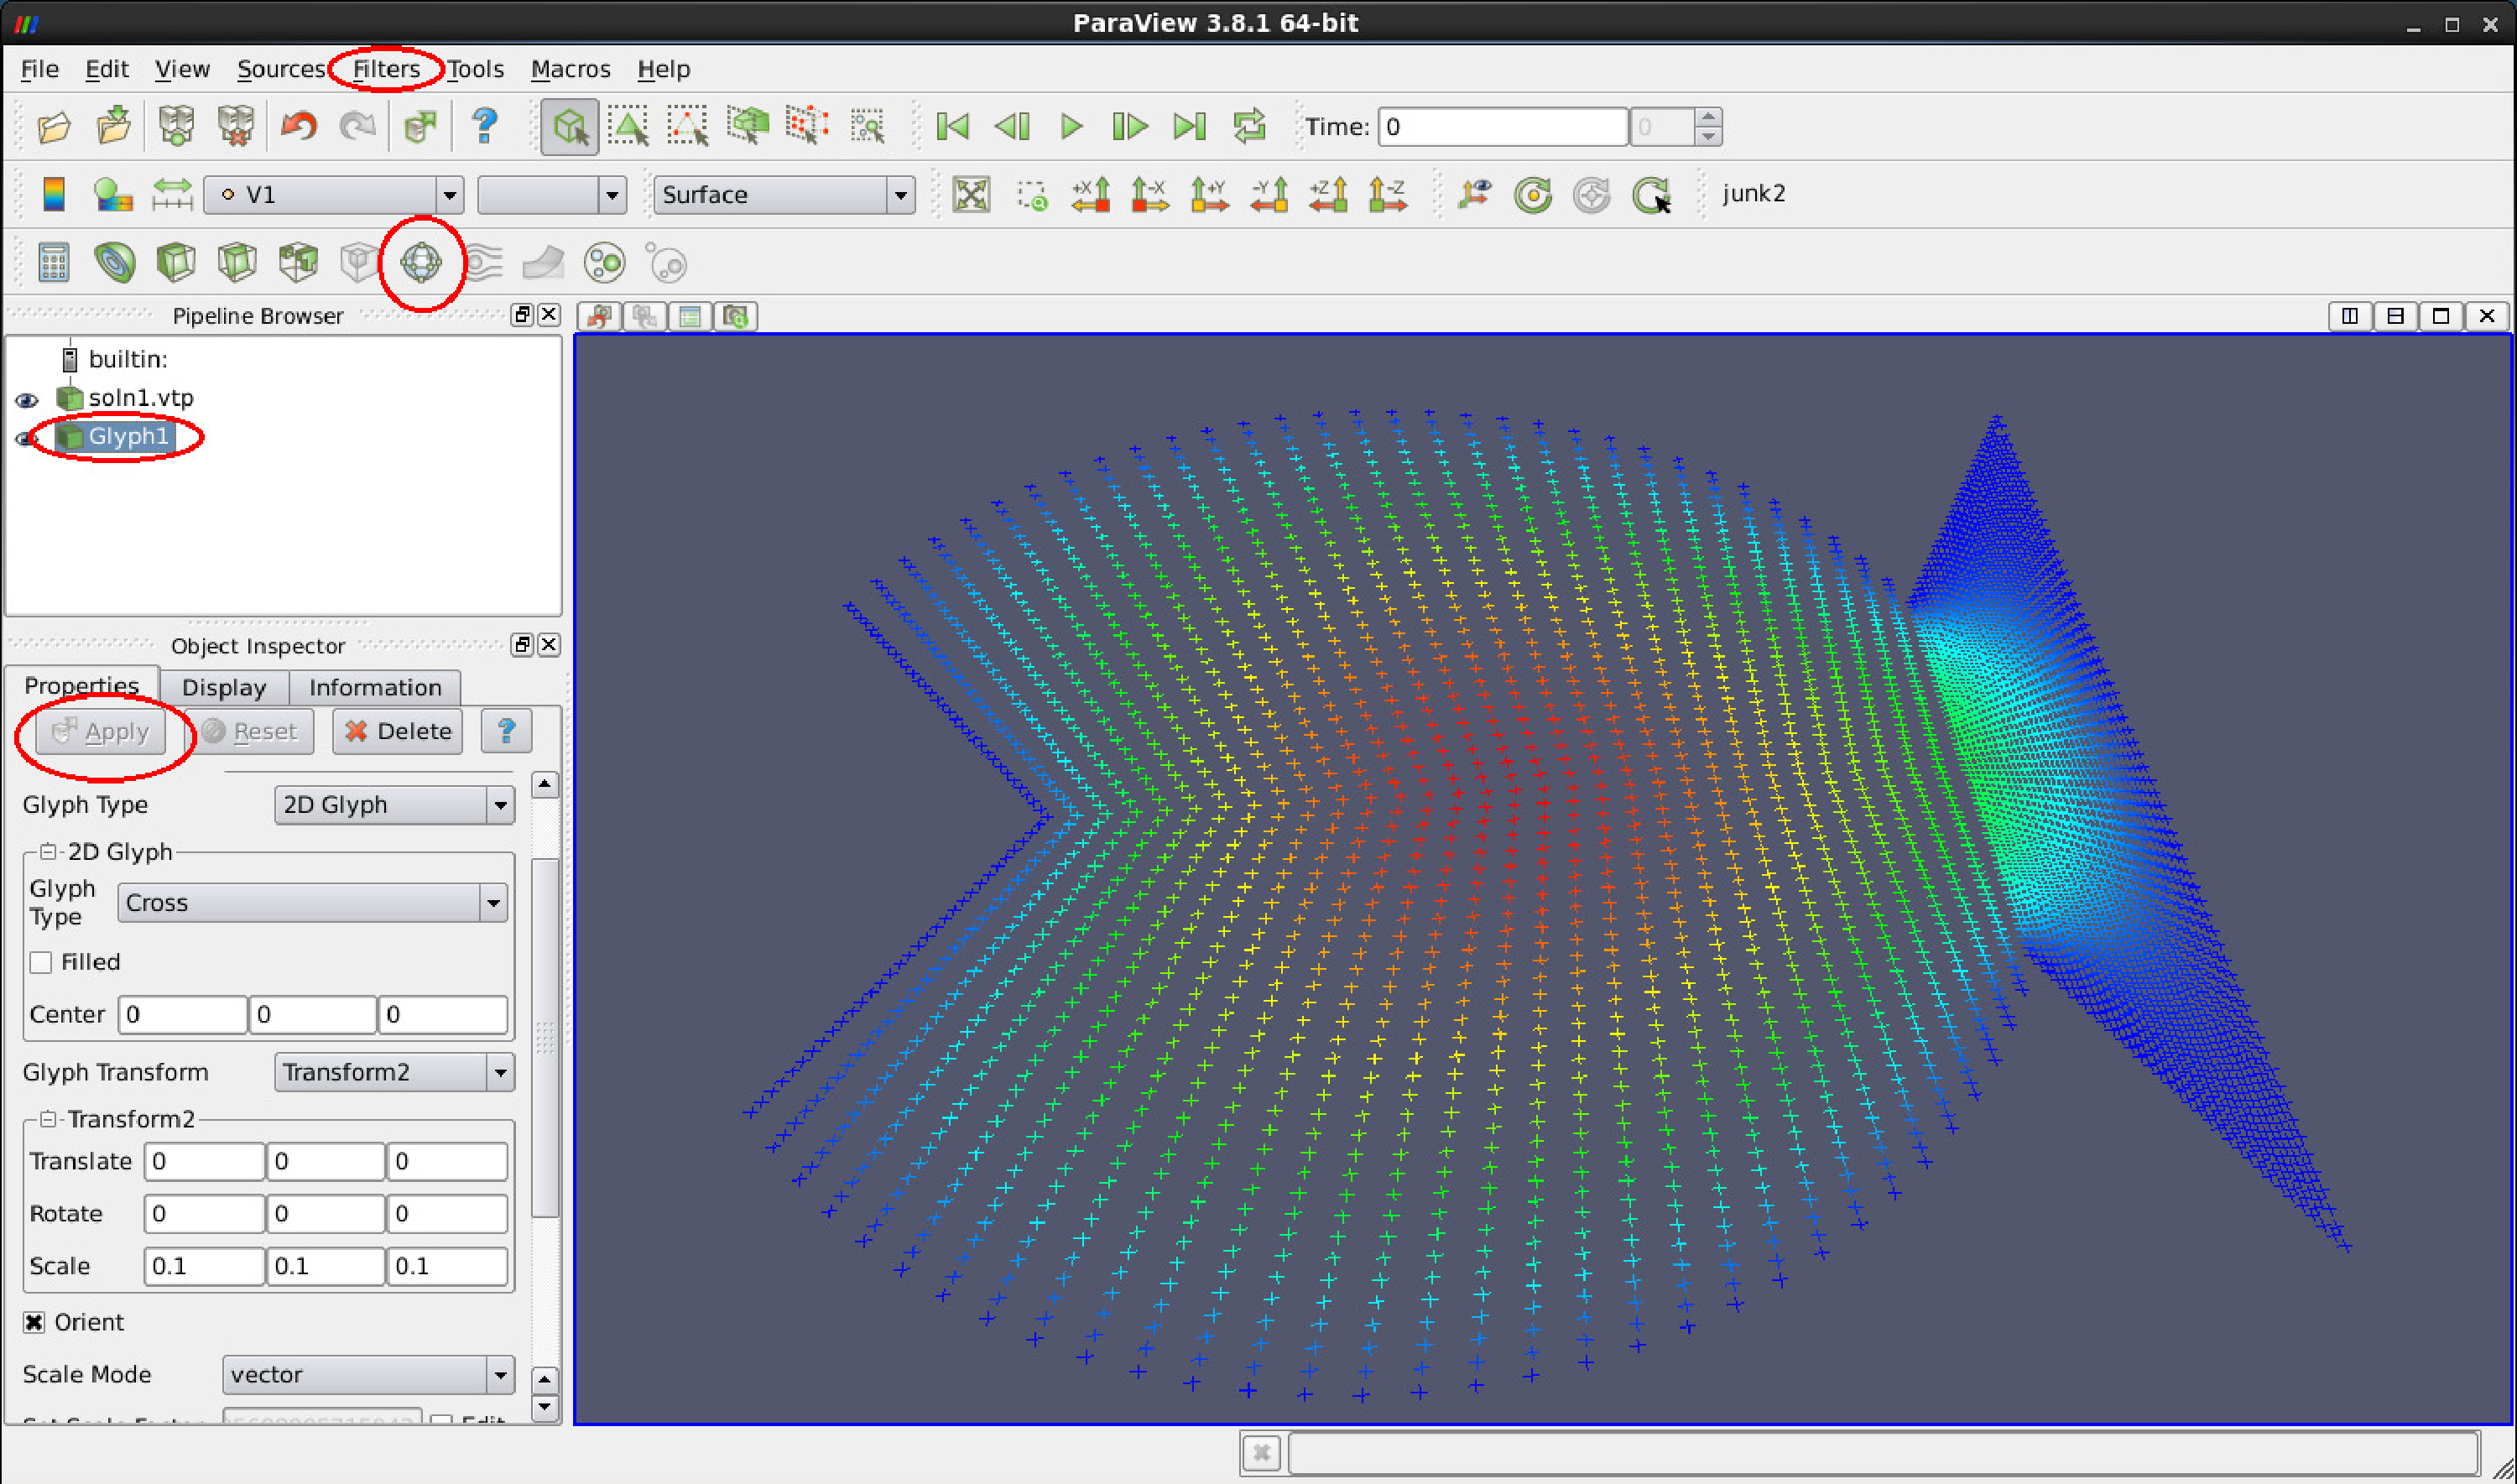
\includegraphics[width=\textwidth]{paraview00}}
\end{DoxyImageNoCaption}
\hypertarget{index_display}{}\subsection{Display your data}\label{index_display}
Here are a few screenshots from a paraview session to get you started. When paraview starts up, you have to select the arrays of values you want to load and click on  
\begin{DoxyImageNoCaption}
  \mbox{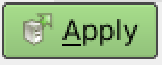
\includegraphics[width=0.07\textwidth]{apply_button}}
\end{DoxyImageNoCaption}
 {\ttfamily Apply\+:} 

 
\begin{DoxyImageNoCaption}
  \mbox{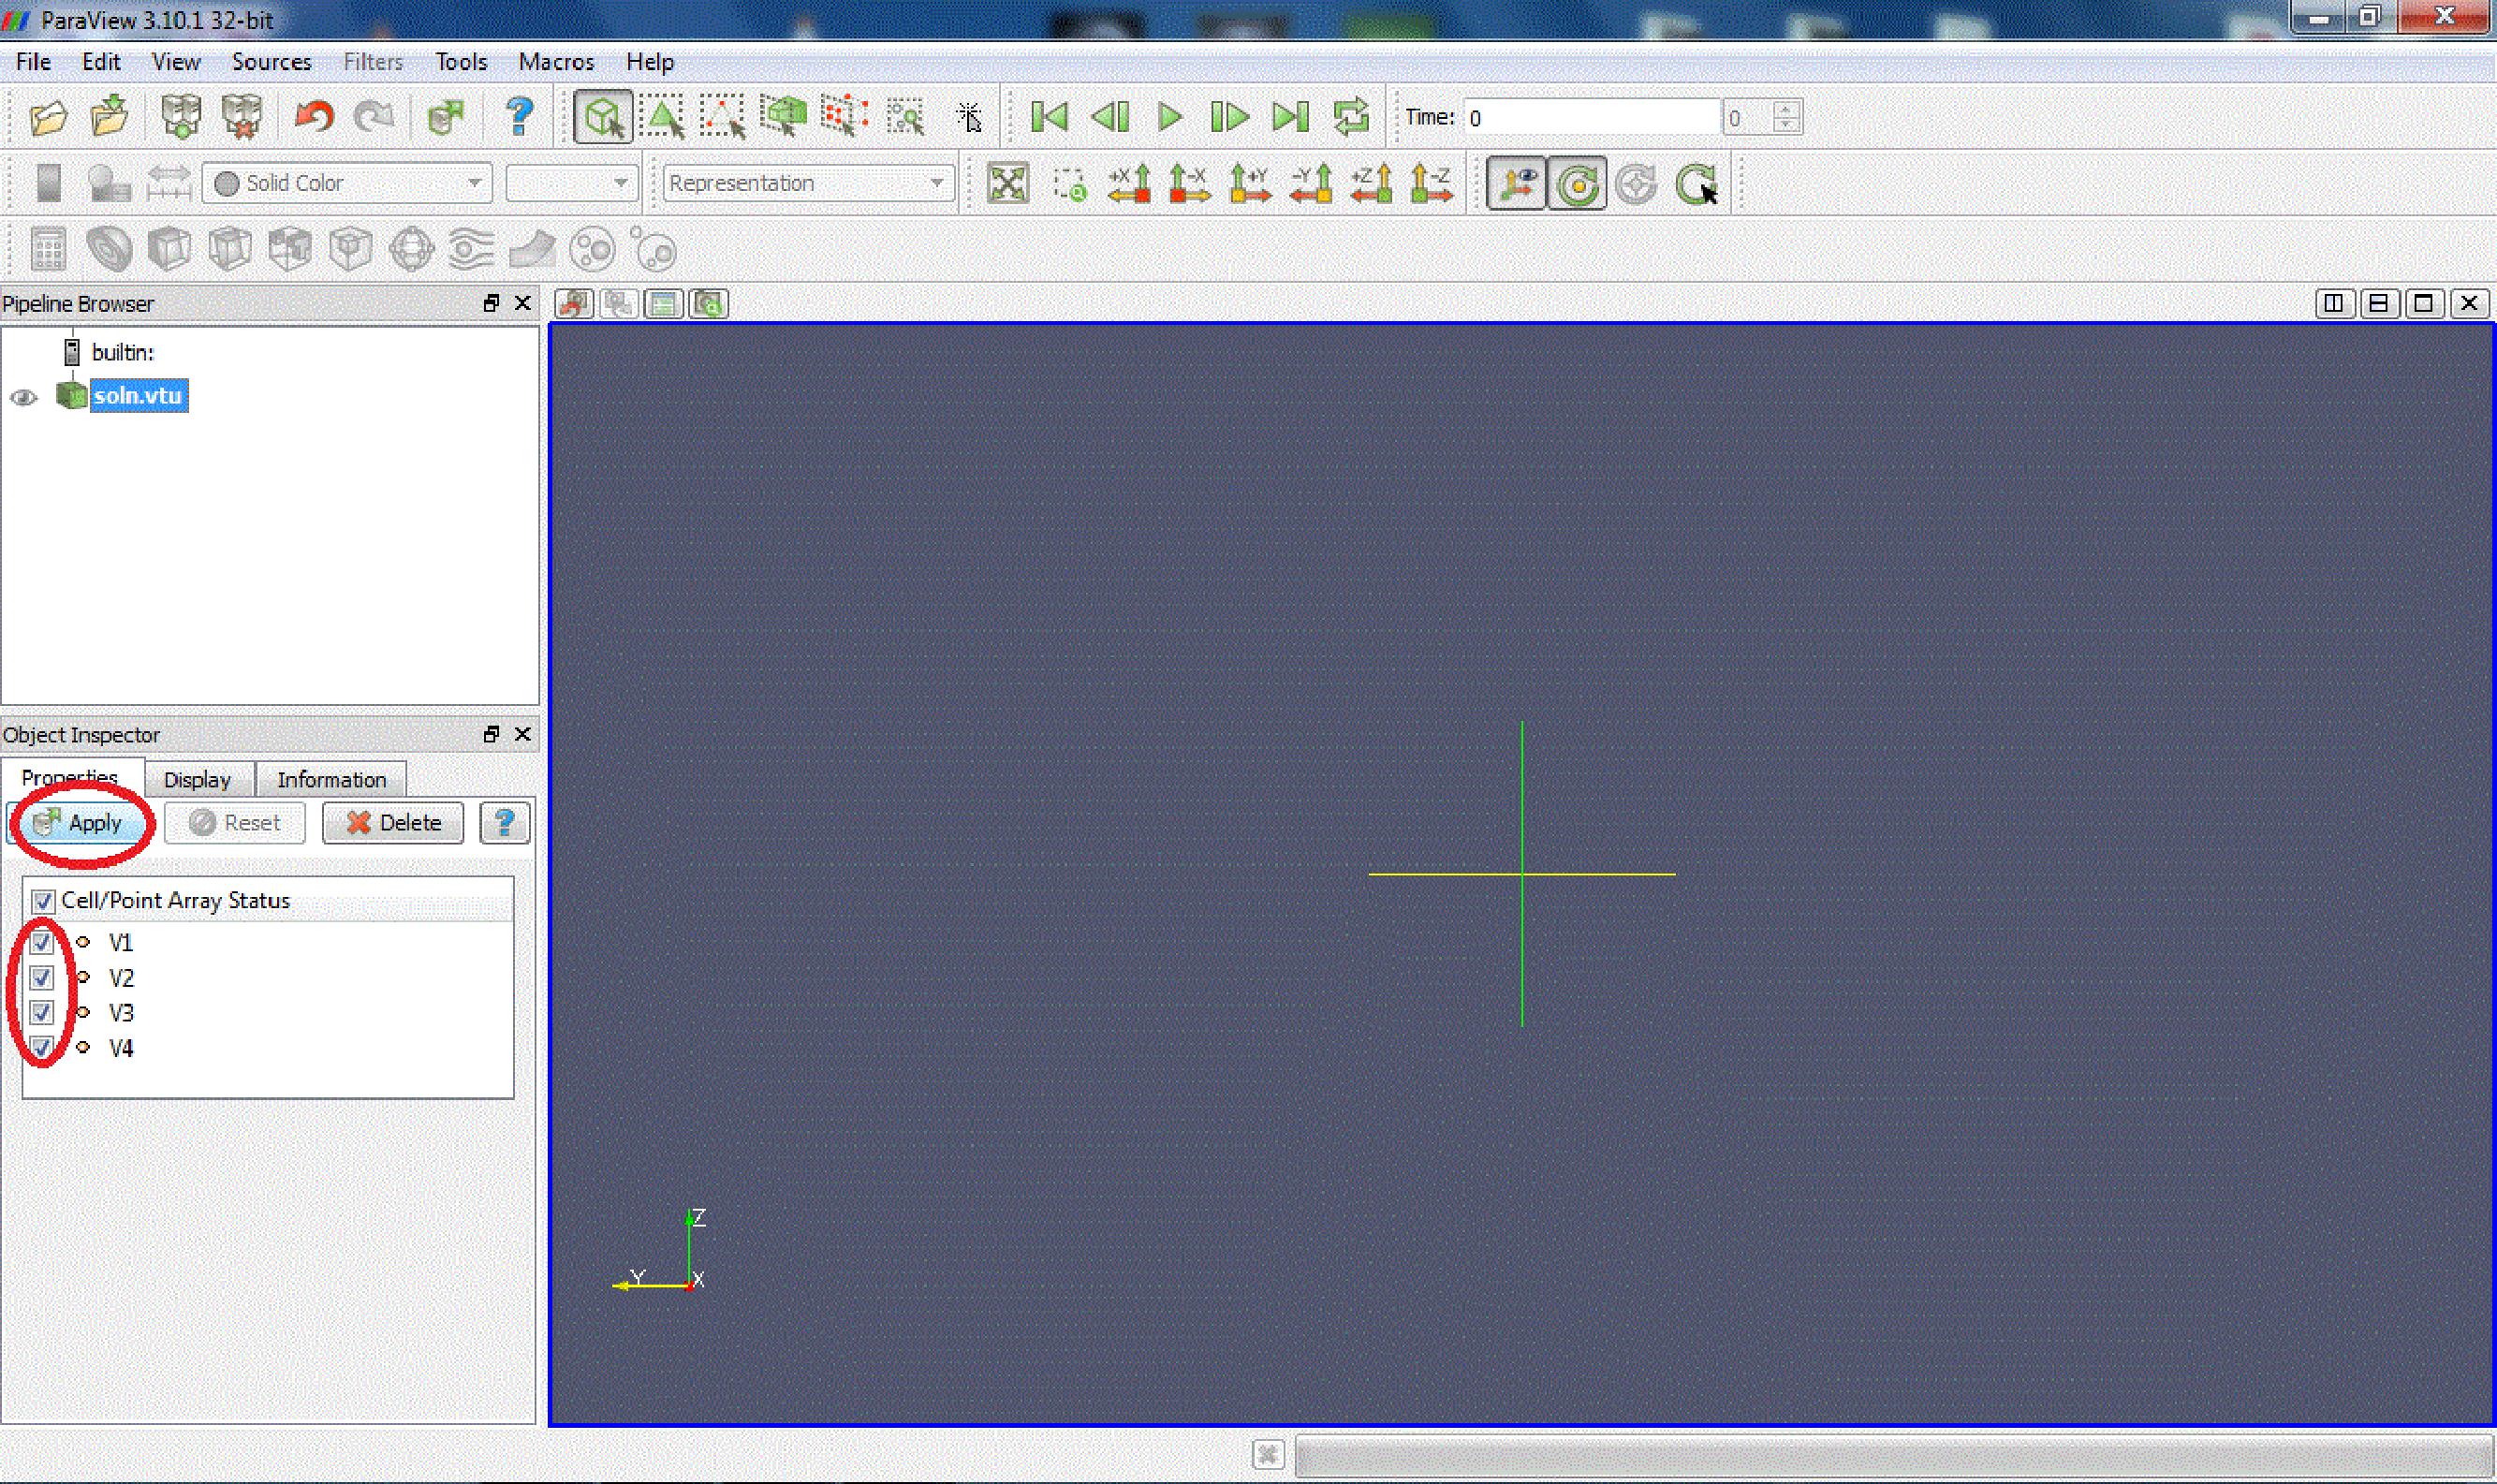
\includegraphics[width=\textwidth]{paraview01}}
\end{DoxyImageNoCaption}


Select the array of values you want to display in the active window (V1, V2, V3...). You can only display one at a time. It is applied on the data set selected in the pipeline\+:

 
\begin{DoxyImageNoCaption}
  \mbox{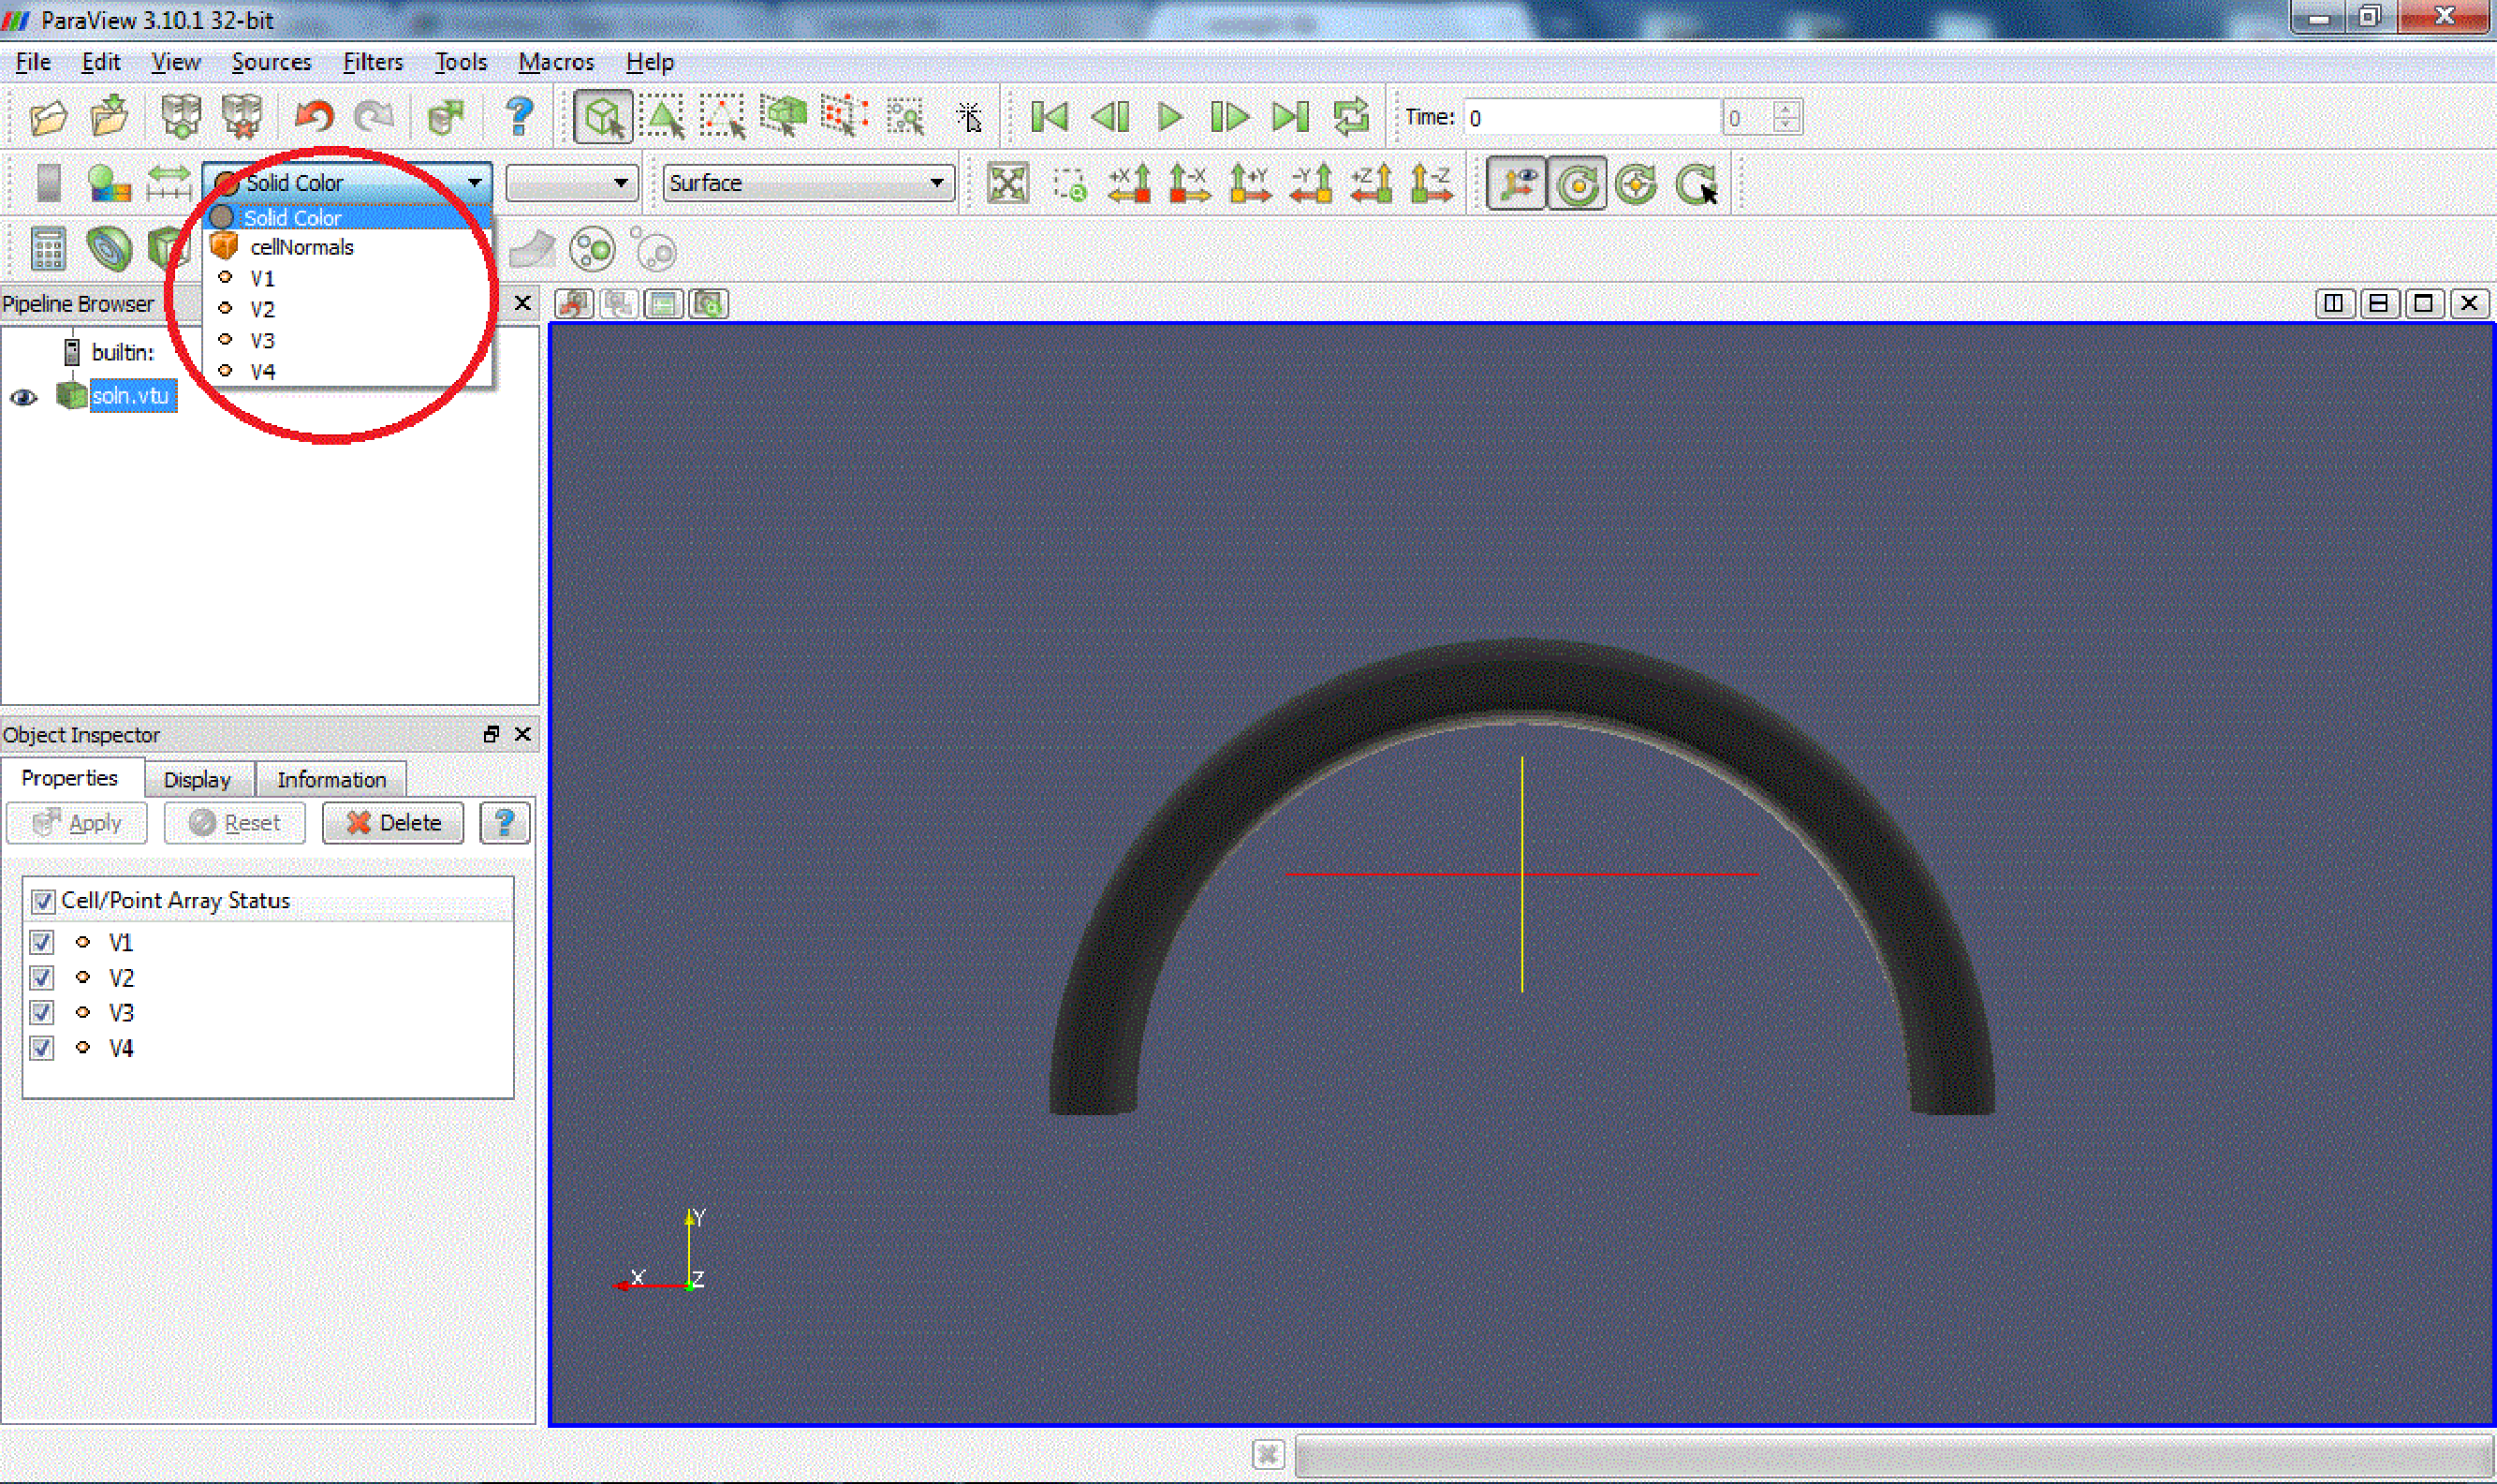
\includegraphics[width=\textwidth]{paraview02}}
\end{DoxyImageNoCaption}


Now choose the plot style of your data. {\ttfamily Outline} display a box containing the data but not the data itself (it\textquotesingle{}s not entirely clear to us why you would want to do this, but...). {\ttfamily Points} and {\ttfamily Wireframe} best suited for 3D computations because they allow you to \char`\"{}see 
through\char`\"{} the data set. {\ttfamily Surface} and {\ttfamily Surface} {\ttfamily With} {\ttfamily Edges} is best suited for 2D computations because only the surface is displayed. Here is a view of the data in {\ttfamily Wireframe} mode\+:

 
\begin{DoxyImageNoCaption}
  \mbox{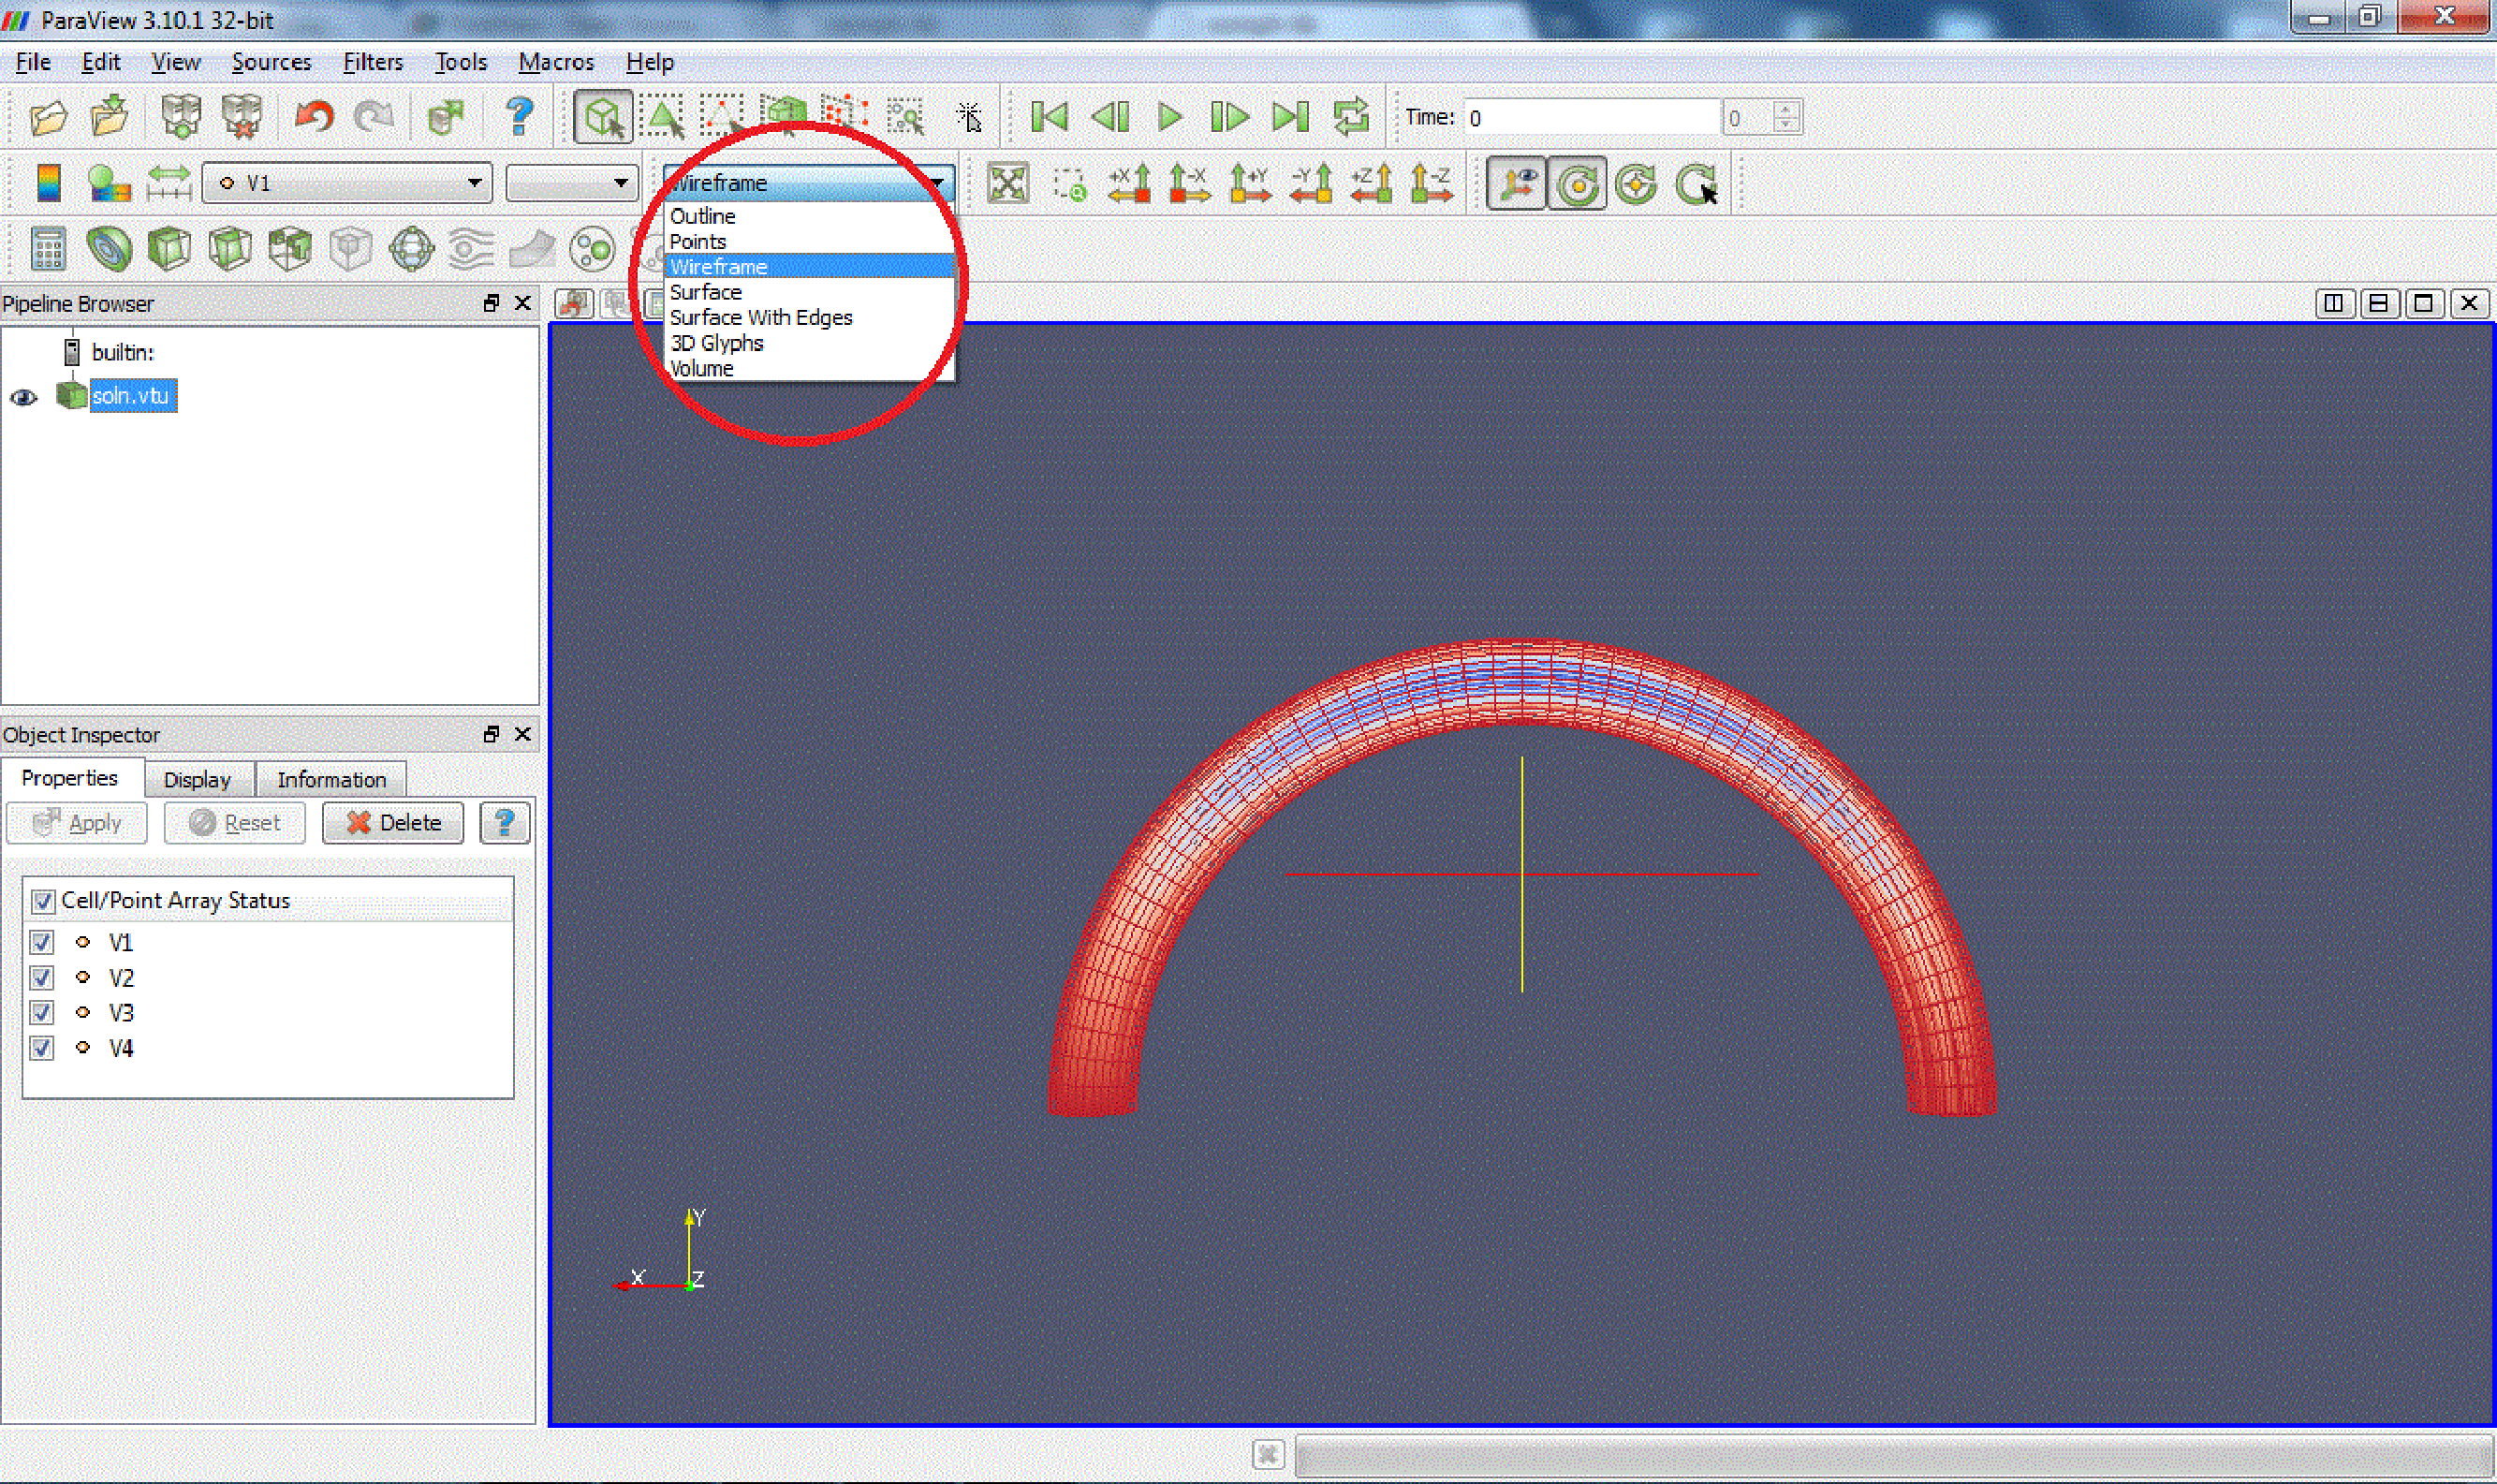
\includegraphics[width=\textwidth]{paraview03}}
\end{DoxyImageNoCaption}


You can move the figure with buttons  
\begin{DoxyImageNoCaption}
  \mbox{
\includegraphics[width=0.30\textwidth]{move_button}}
\end{DoxyImageNoCaption}
 in the toolbar or simply with the mouse\+: \char`\"{}\+Left click + Move\char`\"{} to rotate, \char`\"{}\+Middle click + Move\char`\"{} to move, zoom in with scroll up or \char`\"{}\+Right click + Move up\char`\"{} and zoom out with scroll down or \char`\"{}\+Right click + Move down\char`\"{}.

 
\begin{DoxyImageNoCaption}
  \mbox{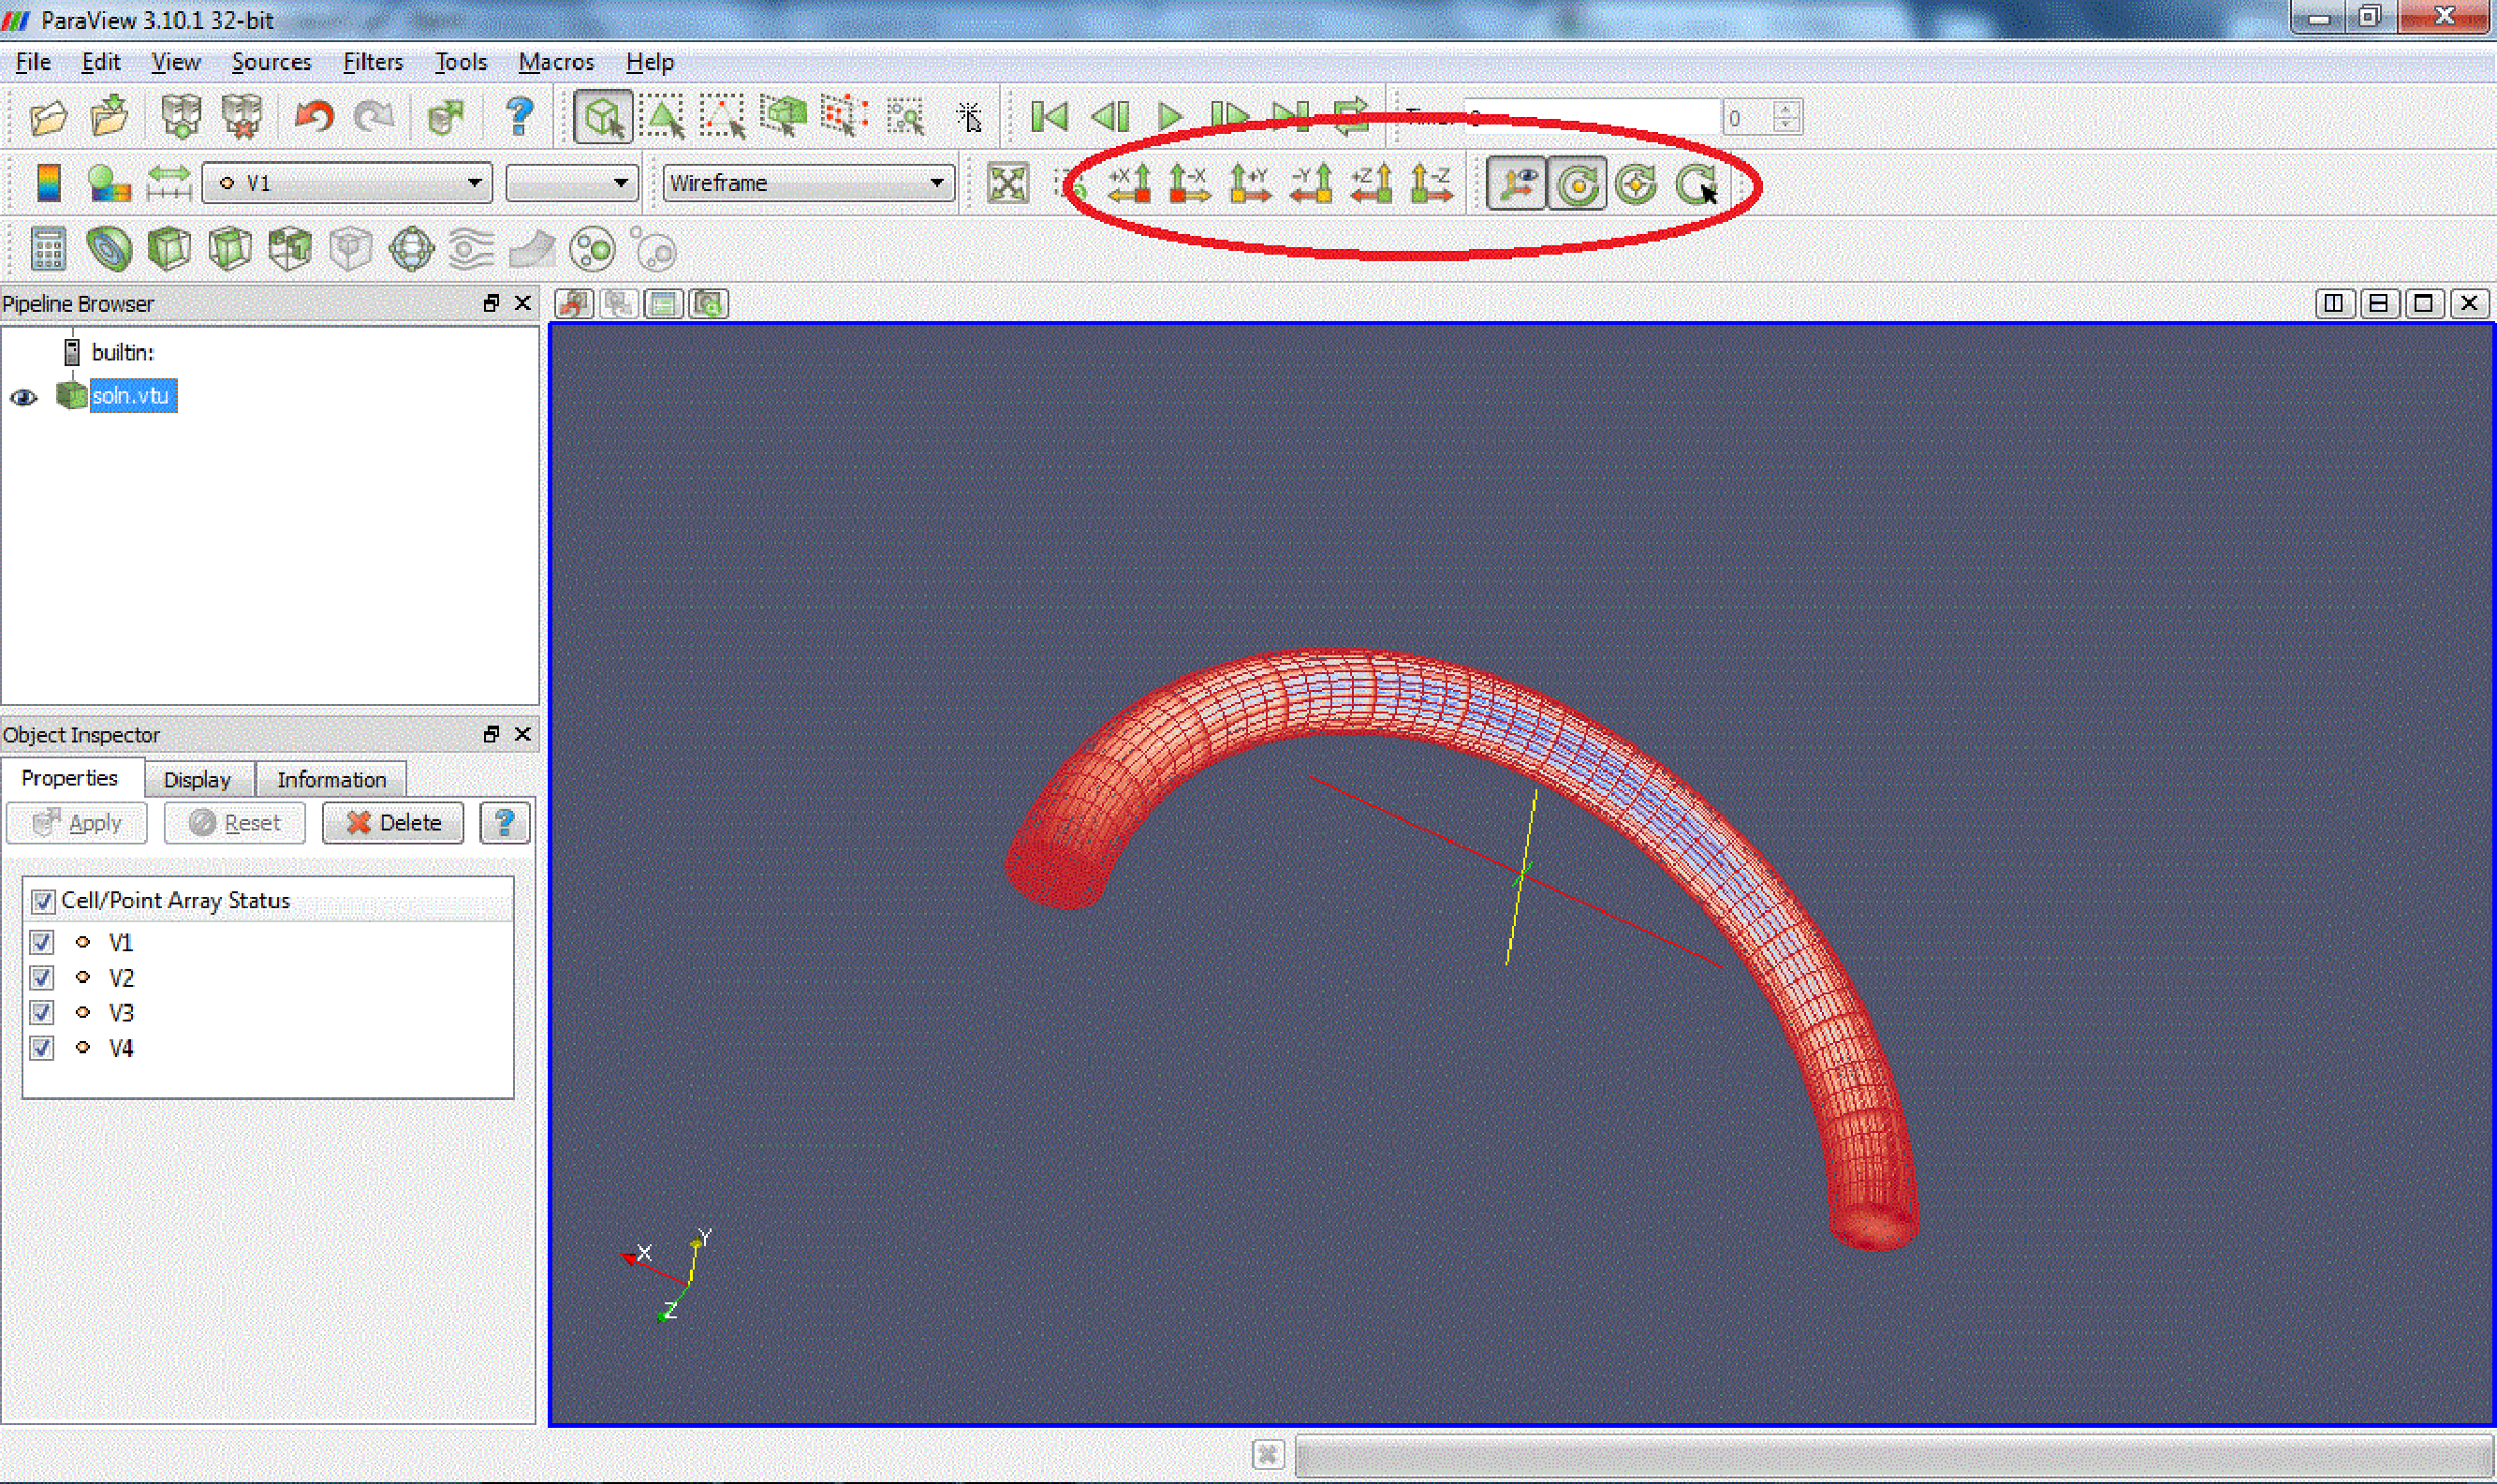
\includegraphics[width=\textwidth]{paraview04}}
\end{DoxyImageNoCaption}


You can also display the colour legend by clicking on  
\begin{DoxyImageNoCaption}
  \mbox{
\includegraphics[width=0.03\textwidth]{legend_button}}
\end{DoxyImageNoCaption}
 , change the display colours (H\+SV, R\+GB, Diverging...) by clicking on  
\begin{DoxyImageNoCaption}
  \mbox{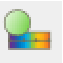
\includegraphics[width=0.03\textwidth]{color_button}}
\end{DoxyImageNoCaption}
 , and rescale the colour scale to data by clicking on  
\begin{DoxyImageNoCaption}
  \mbox{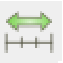
\includegraphics[width=0.03\textwidth]{scale_button}}
\end{DoxyImageNoCaption}
 . Modifying the colour scale is easy\+: add points by clicking on the colour bar to change the distribution of colours or use a logarithmic scale.

 
\begin{DoxyImageNoCaption}
  \mbox{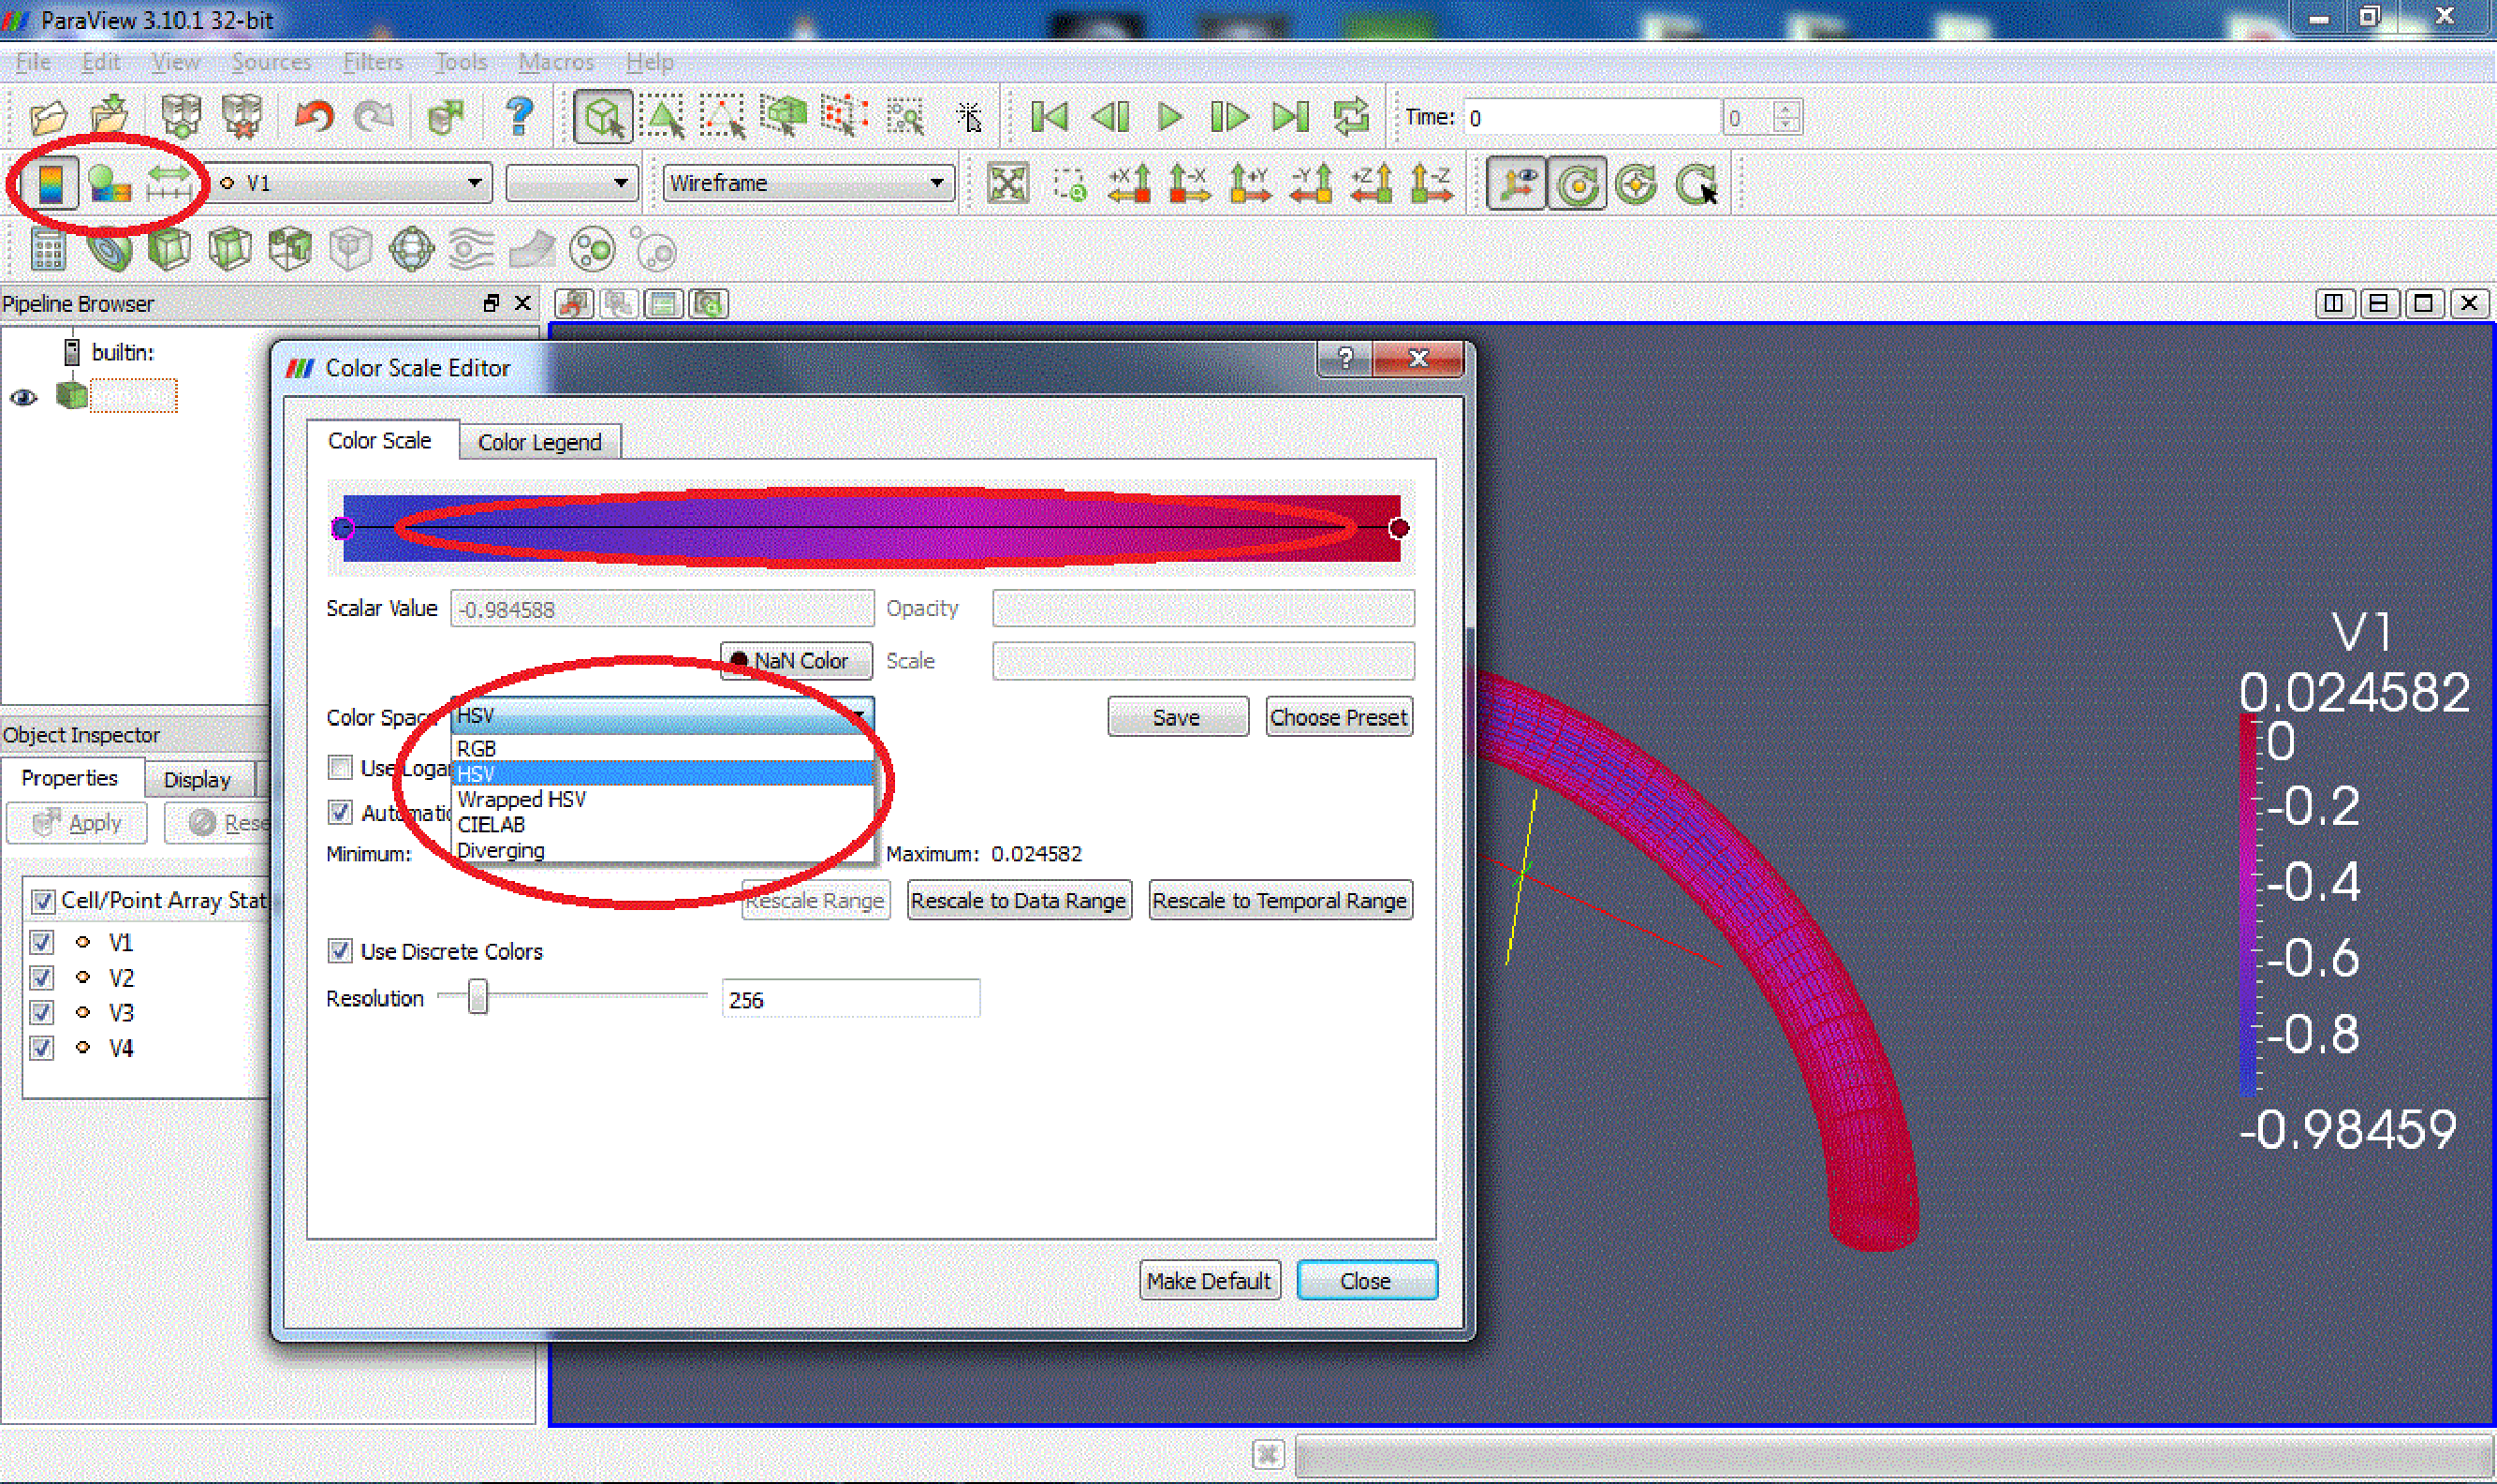
\includegraphics[width=\textwidth]{paraview05}}
\end{DoxyImageNoCaption}


You can split a window by clicking on  
\begin{DoxyImageNoCaption}
  \mbox{
\includegraphics[width=0.07\textwidth]{split_button}}
\end{DoxyImageNoCaption}
 . Clicking on the plot window will make it active. You can switch on/off the display of a pipeline member by clicking on the eye  
\begin{DoxyImageNoCaption}
  \mbox{
\includegraphics[width=0.02\textwidth]{eye_button}}
\end{DoxyImageNoCaption}
 on the left. You can display different values and states in different windows\+:

 
\begin{DoxyImageNoCaption}
  \mbox{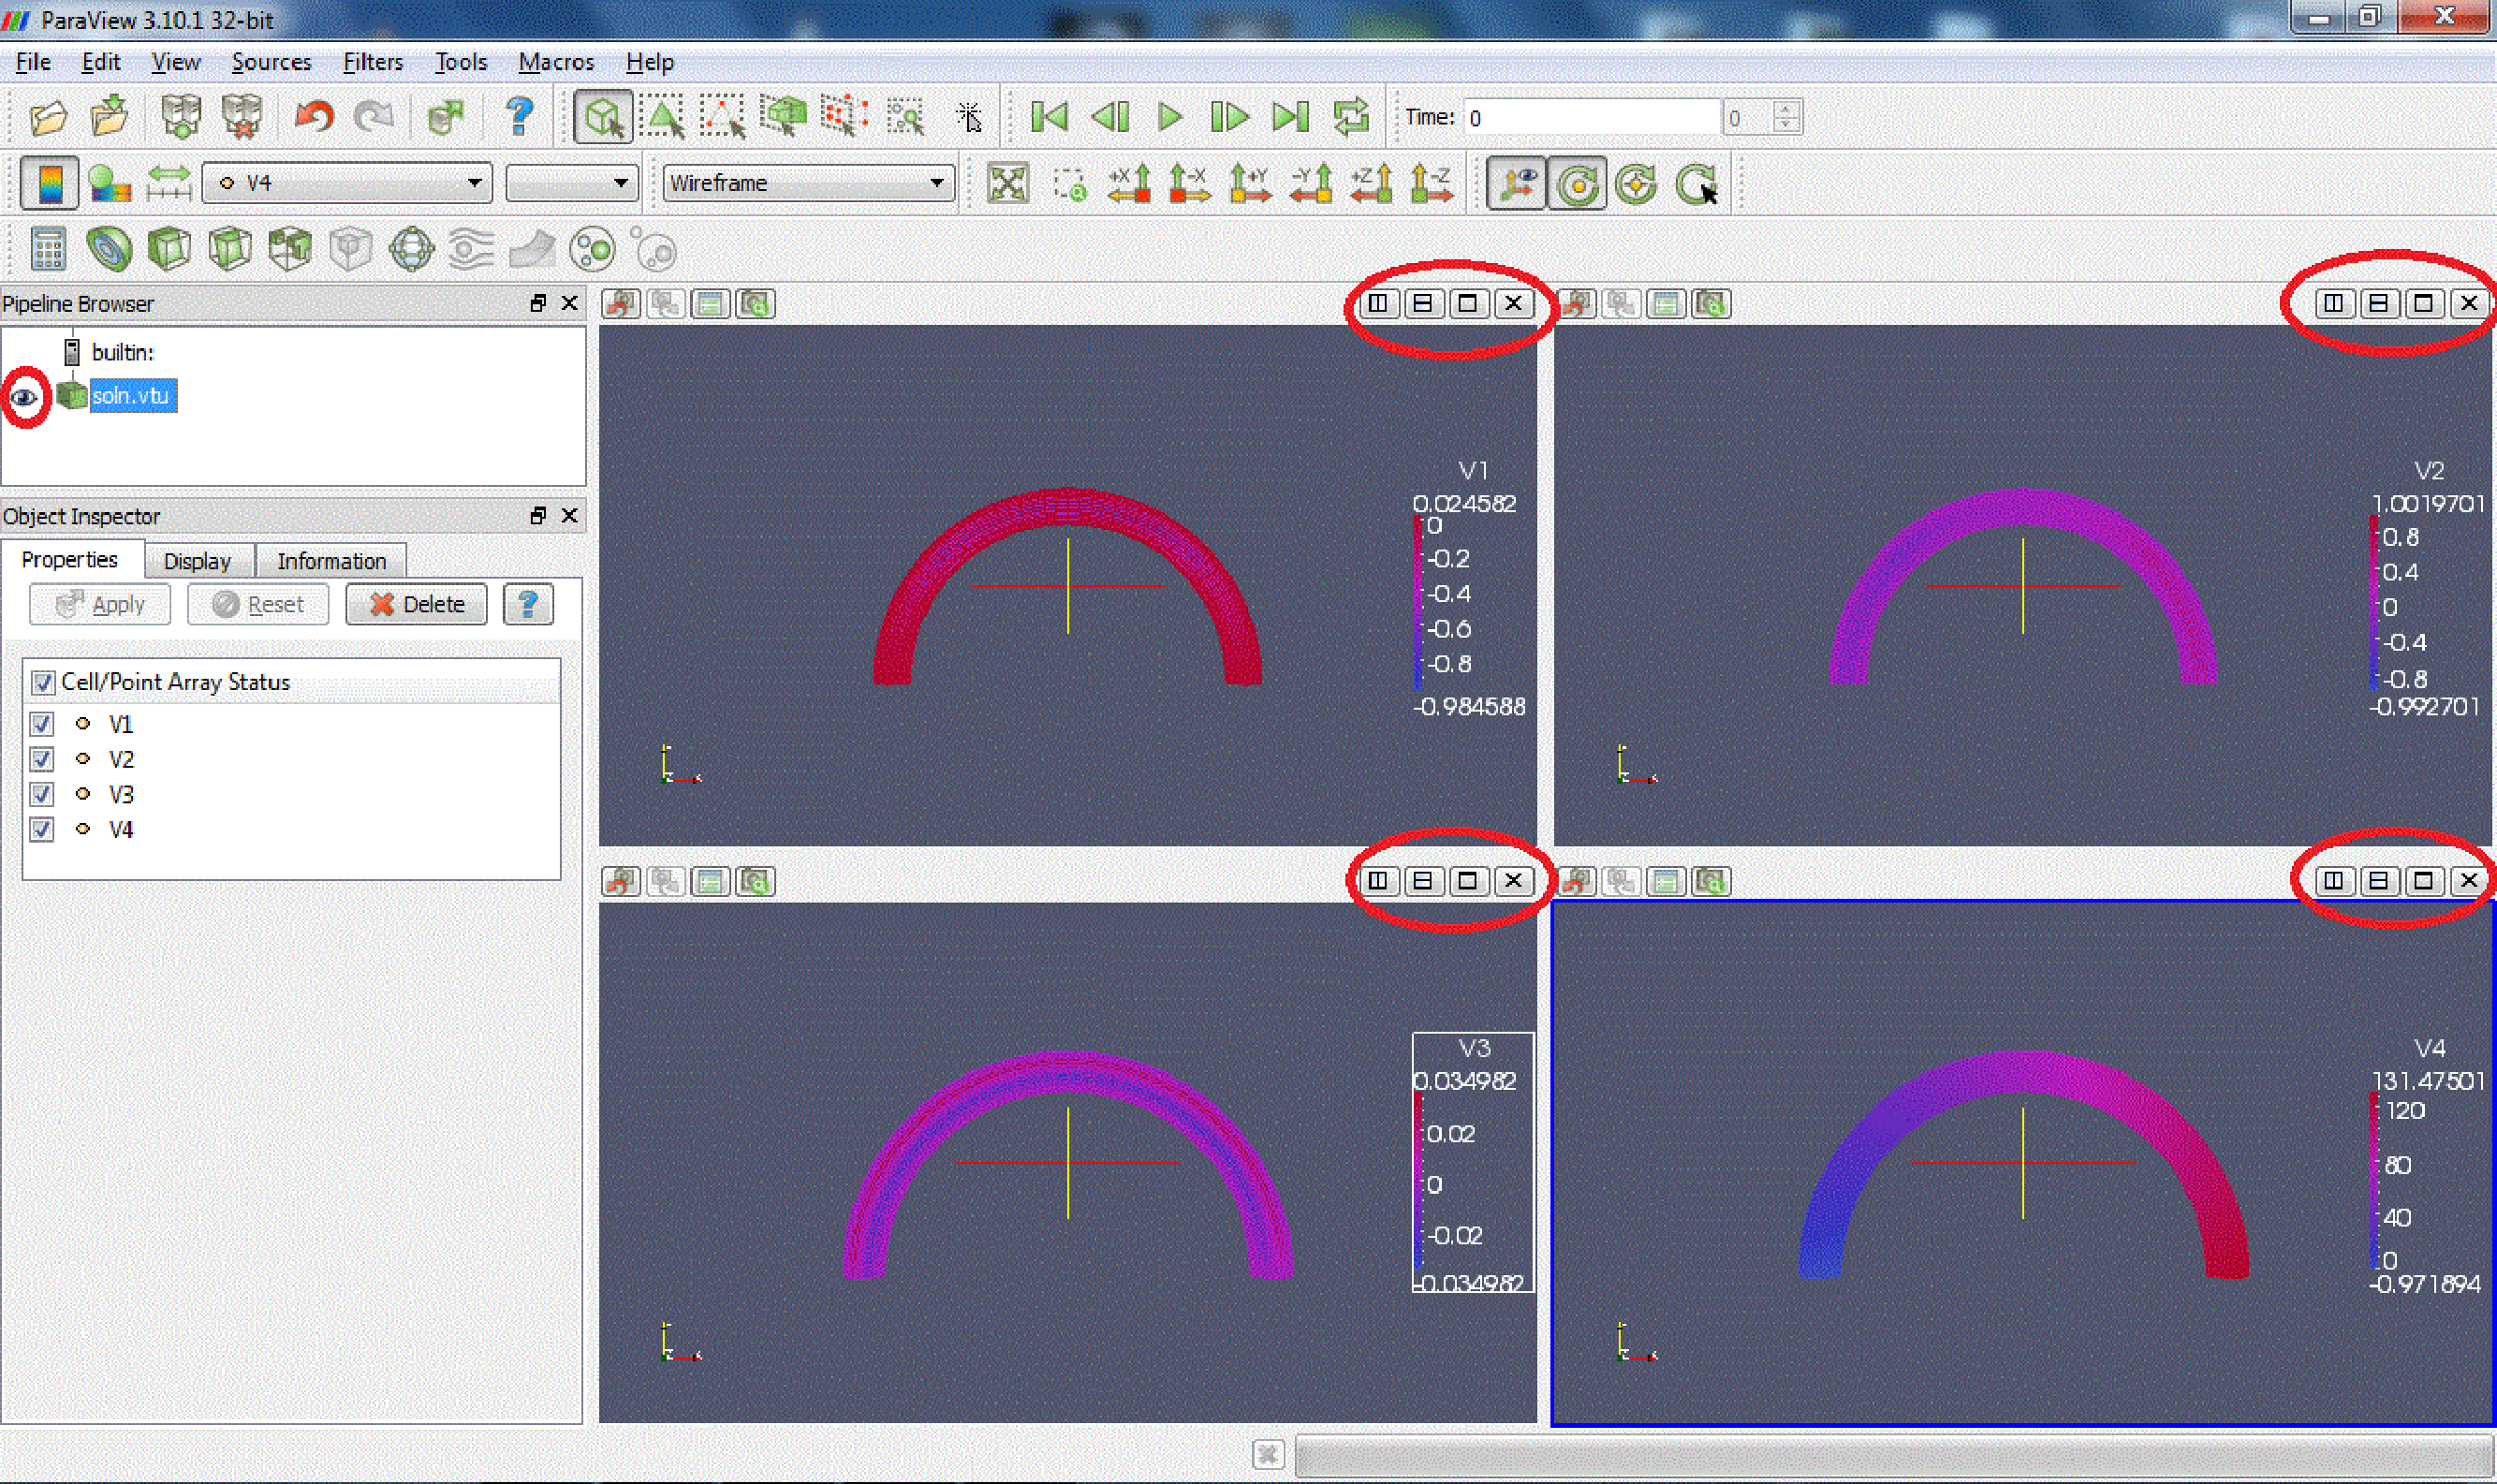
\includegraphics[width=\textwidth]{paraview051}}
\end{DoxyImageNoCaption}




 

\hypertarget{index_py_mult}{}\section{The oomph-\/convert and make\+Pvd scripts for multiple files and animations}\label{index_py_mult}
\hypertarget{index_py_sample_mult}{}\subsection{An example session for data from a serial computation}\label{index_py_sample_mult}
Here is a quick demonstration of {\ttfamily oomph-\/convert} and {\ttfamily make\+Pvd} scripts in action


\begin{DoxyEnumerate}
\item Add {\ttfamily oomph-\/lib\textquotesingle{}s} bin directory to your path (in the example shown here, {\ttfamily oomph-\/lib} is installed in the directory {\ttfamily /home/mheil/version185/oomph})\+: ~\newline
~\newline

\begin{DoxyCode}
biowulf: 10:31:50$ PATH=$PATH:/home/mheil/version185/oomph/bin
\end{DoxyCode}
 ~\newline

\item Here is what\textquotesingle{}s in the current directory at the moment\+: {\ttfamily soln}?. {\ttfamily dat} are the {\ttfamily oomph-\/lib} output files that illustrate the progress of the mesh adaptation during \href{../../poisson/fish_poisson/html/index.html}{\tt the adaptive solution of a Poisson equation in a fish-\/shaped domain.} ~\newline
~\newline

\begin{DoxyCode}
biowulf: 11:05:10$ ll
total 824
-rw-r--r--    1 mheil    users        2292 May 21 09:19 soln0.dat
-rw-r--r--    1 mheil    users      176776 May 21 09:19 soln1.dat
-rw-r--r--    1 mheil    users      278117 May 21 09:19 soln2.dat
-rw-r--r--    1 mheil    users      367408 May 21 09:19 soln3.dat
\end{DoxyCode}
 ~\newline

\item Run {\ttfamily oomph-\/convert} on all files (the -\/z option adds zeroes to the numbers -- this is only required if the files are to combined into an animation by paraview) ~\newline
~\newline

\begin{DoxyCode}
biowulf: 11:16:13$ oomph-convert -z soln*.dat


-- Processing soln0.dat
  oomph-convert.py, ver. 20110615
Parse input file \textcolor{keywordflow}{for} Tecplot zones........done
  0 lines ignored    
Write nodal coordinates...................done
Write cell connectivity..................done
Write cell offsets.......................done
Write cell types.........................done
Write field 01/01.........................done
  Conversion done in 0 seconds
  Output file name: soln00000.vtu 


-- Processing soln1.dat
  oomph-convert.py, ver. 20110615
Parse input file \textcolor{keywordflow}{for} Tecplot zones........done
  0 lines ignored    
Write nodal coordinates...................done
Write cell connectivity..................done
Write cell offsets.......................done
Write cell types.........................done
Write field 01/01.........................done
  Conversion done in 0 seconds
  Output file name: soln00001.vtu 


[further output suppressed]
\end{DoxyCode}
 ~\newline

\item We now have the corresponding {\ttfamily $\ast$} {\ttfamily }.vtu files ~\newline
~\newline

\begin{DoxyCode}
biowulf: 12:37:05$ ll
total 2568
-rw-r--r--    1 mheil    users        5979 Jun 21 12:37 soln00000.vtu
-rw-r--r--    1 mheil    users      377490 Jun 21 12:37 soln00001.vtu
-rw-r--r--    1 mheil    users      592990 Jun 21 12:37 soln00002.vtu
-rw-r--r--    1 mheil    users      789325 Jun 21 12:37 soln00003.vtu
-rw-r--r--    1 mheil    users        2292 Jun 21 09:19 soln0.dat
-rw-r--r--    1 mheil    users      176776 Jun 21 09:19 soln1.dat
-rw-r--r--    1 mheil    users      278117 Jun 21 09:19 soln2.dat
-rw-r--r--    1 mheil    users      367408 Jun 21 09:19 soln3.dat
\end{DoxyCode}
 ~\newline
 These {\ttfamily $\ast$} {\ttfamily }.vtu files can be displayed individually as discussed above. ~\newline
~\newline

\item To produce an animation of the results with paraview, create a {\ttfamily $\ast$} {\ttfamily }.pvd file using {\ttfamily make\+Pvd} ~\newline
~\newline
 
\begin{DoxyCode}
biowulf: 12:40:56$ makePvd soln mysoln.pvd
--> File mysoln.pvd created
\end{DoxyCode}
 ~\newline
~\newline

\item ...and visualise it\+: ~\newline
~\newline

\begin{DoxyCode}
biowulf: 12:42:08$ paraview --data=mysoln.pvd  
\end{DoxyCode}

\end{DoxyEnumerate}



 

\hypertarget{index_screenshots_mult}{}\subsection{Screenshots from the paraview session}\label{index_screenshots_mult}
Here\textquotesingle{}s a screenshot from the paraview session\+: once the {\ttfamily $\ast$} {\ttfamily }.pvd file is loaded you can customise the plot style as discussed in the previous example, and then use the  
\begin{DoxyImageNoCaption}
  \mbox{
\includegraphics[width=0.1\textwidth]{play_buttons}}
\end{DoxyImageNoCaption}
 {\ttfamily Play/\+Stop/}... buttons to animate the progress of the mesh adaptation.

 
\begin{DoxyImageNoCaption}
  \mbox{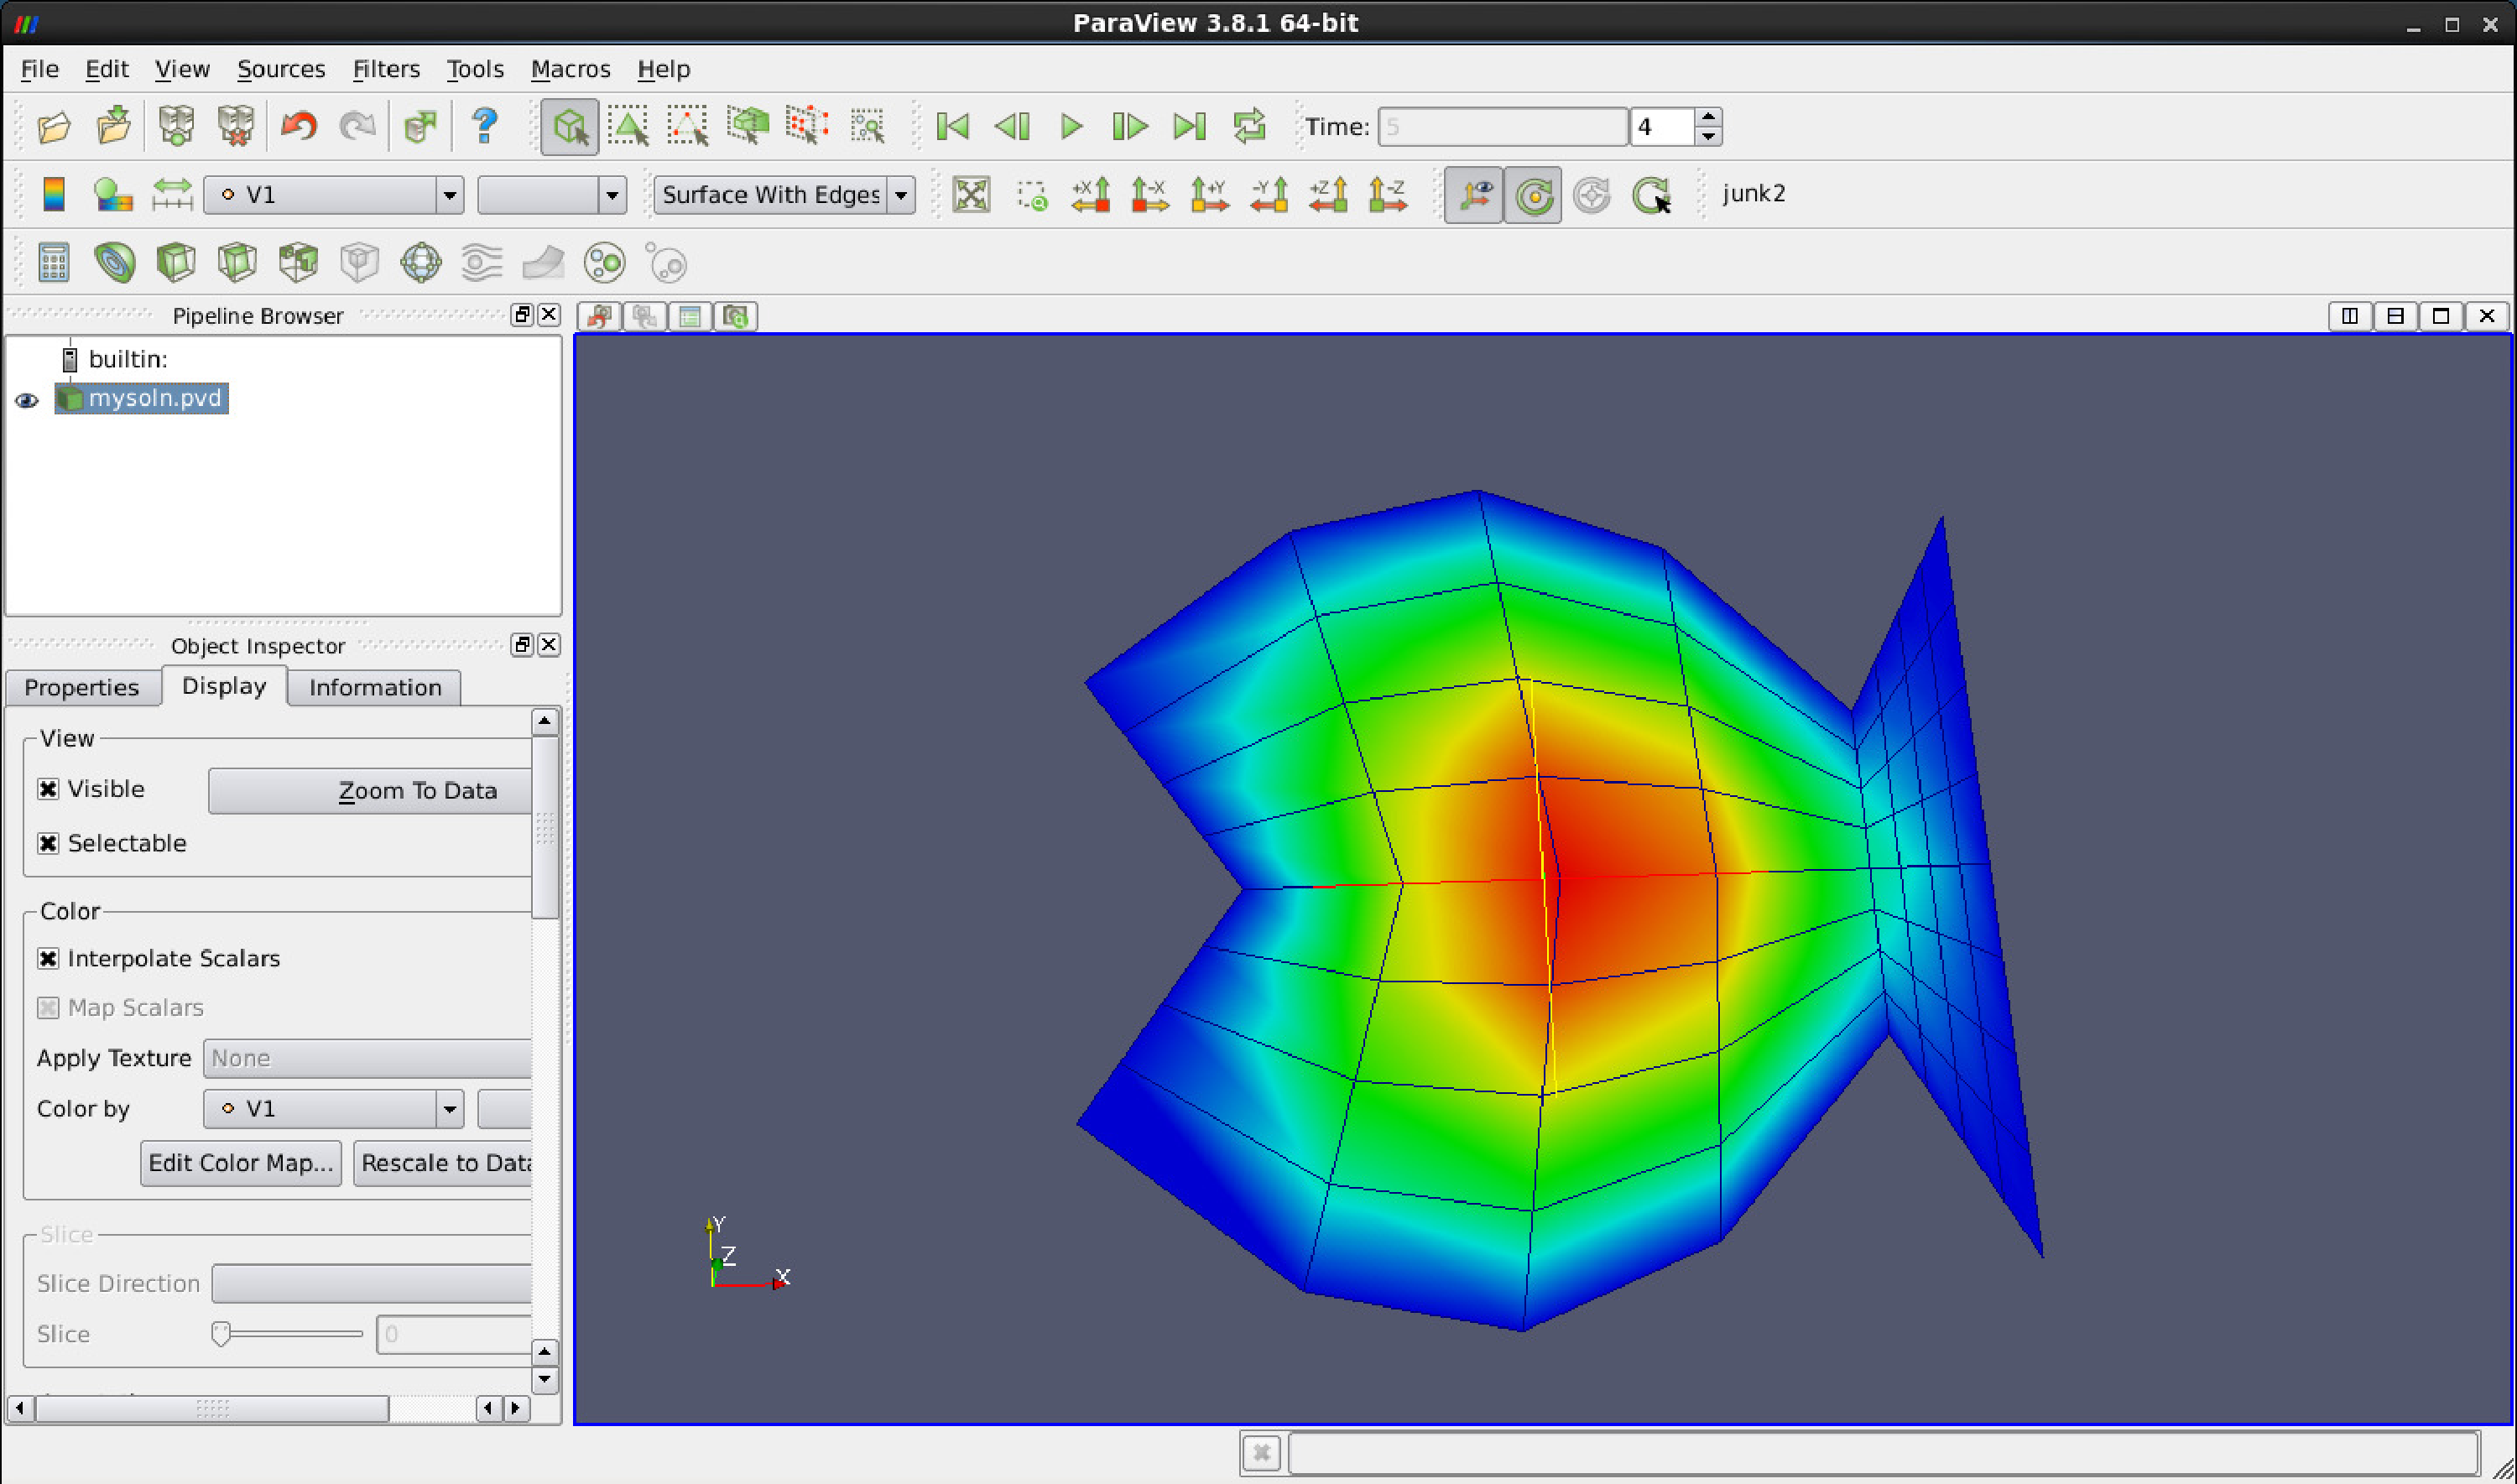
\includegraphics[width=\textwidth]{paraview_animation_select}}
\end{DoxyImageNoCaption}




 

\hypertarget{index_py_sample_mult_par}{}\subsection{An example session for data from a parallel computation}\label{index_py_sample_mult_par}
{\ttfamily oomph-\/lib} typically outputs results from parallel (distributed) computations on a processor-\/by-\/processor basis, resulting in filenames of the form 
\begin{DoxyCode}
soln\_proc0\_0.dat                \(\backslash\) 
soln\_proc1\_0.dat                | 
        :                       | Data \textcolor{keywordflow}{for} timestep 0 
soln\_proc[NPROC-1]\_0.dat        / 
        

soln\_proc0\_1.dat                \(\backslash\) 
soln\_proc1\_1.dat                | 
        :                       | Data \textcolor{keywordflow}{for} timestep 1 
soln\_proc[NPROC-1]\_1.dat,       /

        :
\end{DoxyCode}
 where N\+P\+R\+OC is the number of processors. An animation of such data obviously requires the output from different processors (but for the the same timestep) to be combined. Provided, the filenames have the pattern 
\begin{DoxyCode}
[stem]proc[processor\_number]\_[timestep\_number].dat
\end{DoxyCode}
 (note the \char`\"{}proc\char`\"{} and \char`\"{}\+\_\+\char`\"{}, both of which are required), the pvd file can be generated by first processing the files with {\ttfamily oomph-\/convert}, 
\begin{DoxyCode}
oomph-convert -z [stem]proc* 
\end{DoxyCode}
 followed by 
\begin{DoxyCode}
makePvd [NPROC] [stem] myplot.pvd 
\end{DoxyCode}
 So, for the files listed above, to produce a pvd file that contains data from a computation with four processors the commands 
\begin{DoxyCode}
biowulf: 12:40:56$ oomph-convert soln\_proc*
\end{DoxyCode}
 followed by 
\begin{DoxyCode}
biowulf: 12:40:59$ makePvd 4 soln\_ soln.pvd 
\end{DoxyCode}
 would create the file soln.\+pvd from which paraview can create an animation of the solution.



 

\hypertarget{index_filters}{}\section{Data analysis with filters}\label{index_filters}
In order to analyse the data, we can apply filters. Some filters are accessible directly via the navigation bar; a full list is available in the {\ttfamily Filters} menu\+:

 
\begin{DoxyImageNoCaption}
  \mbox{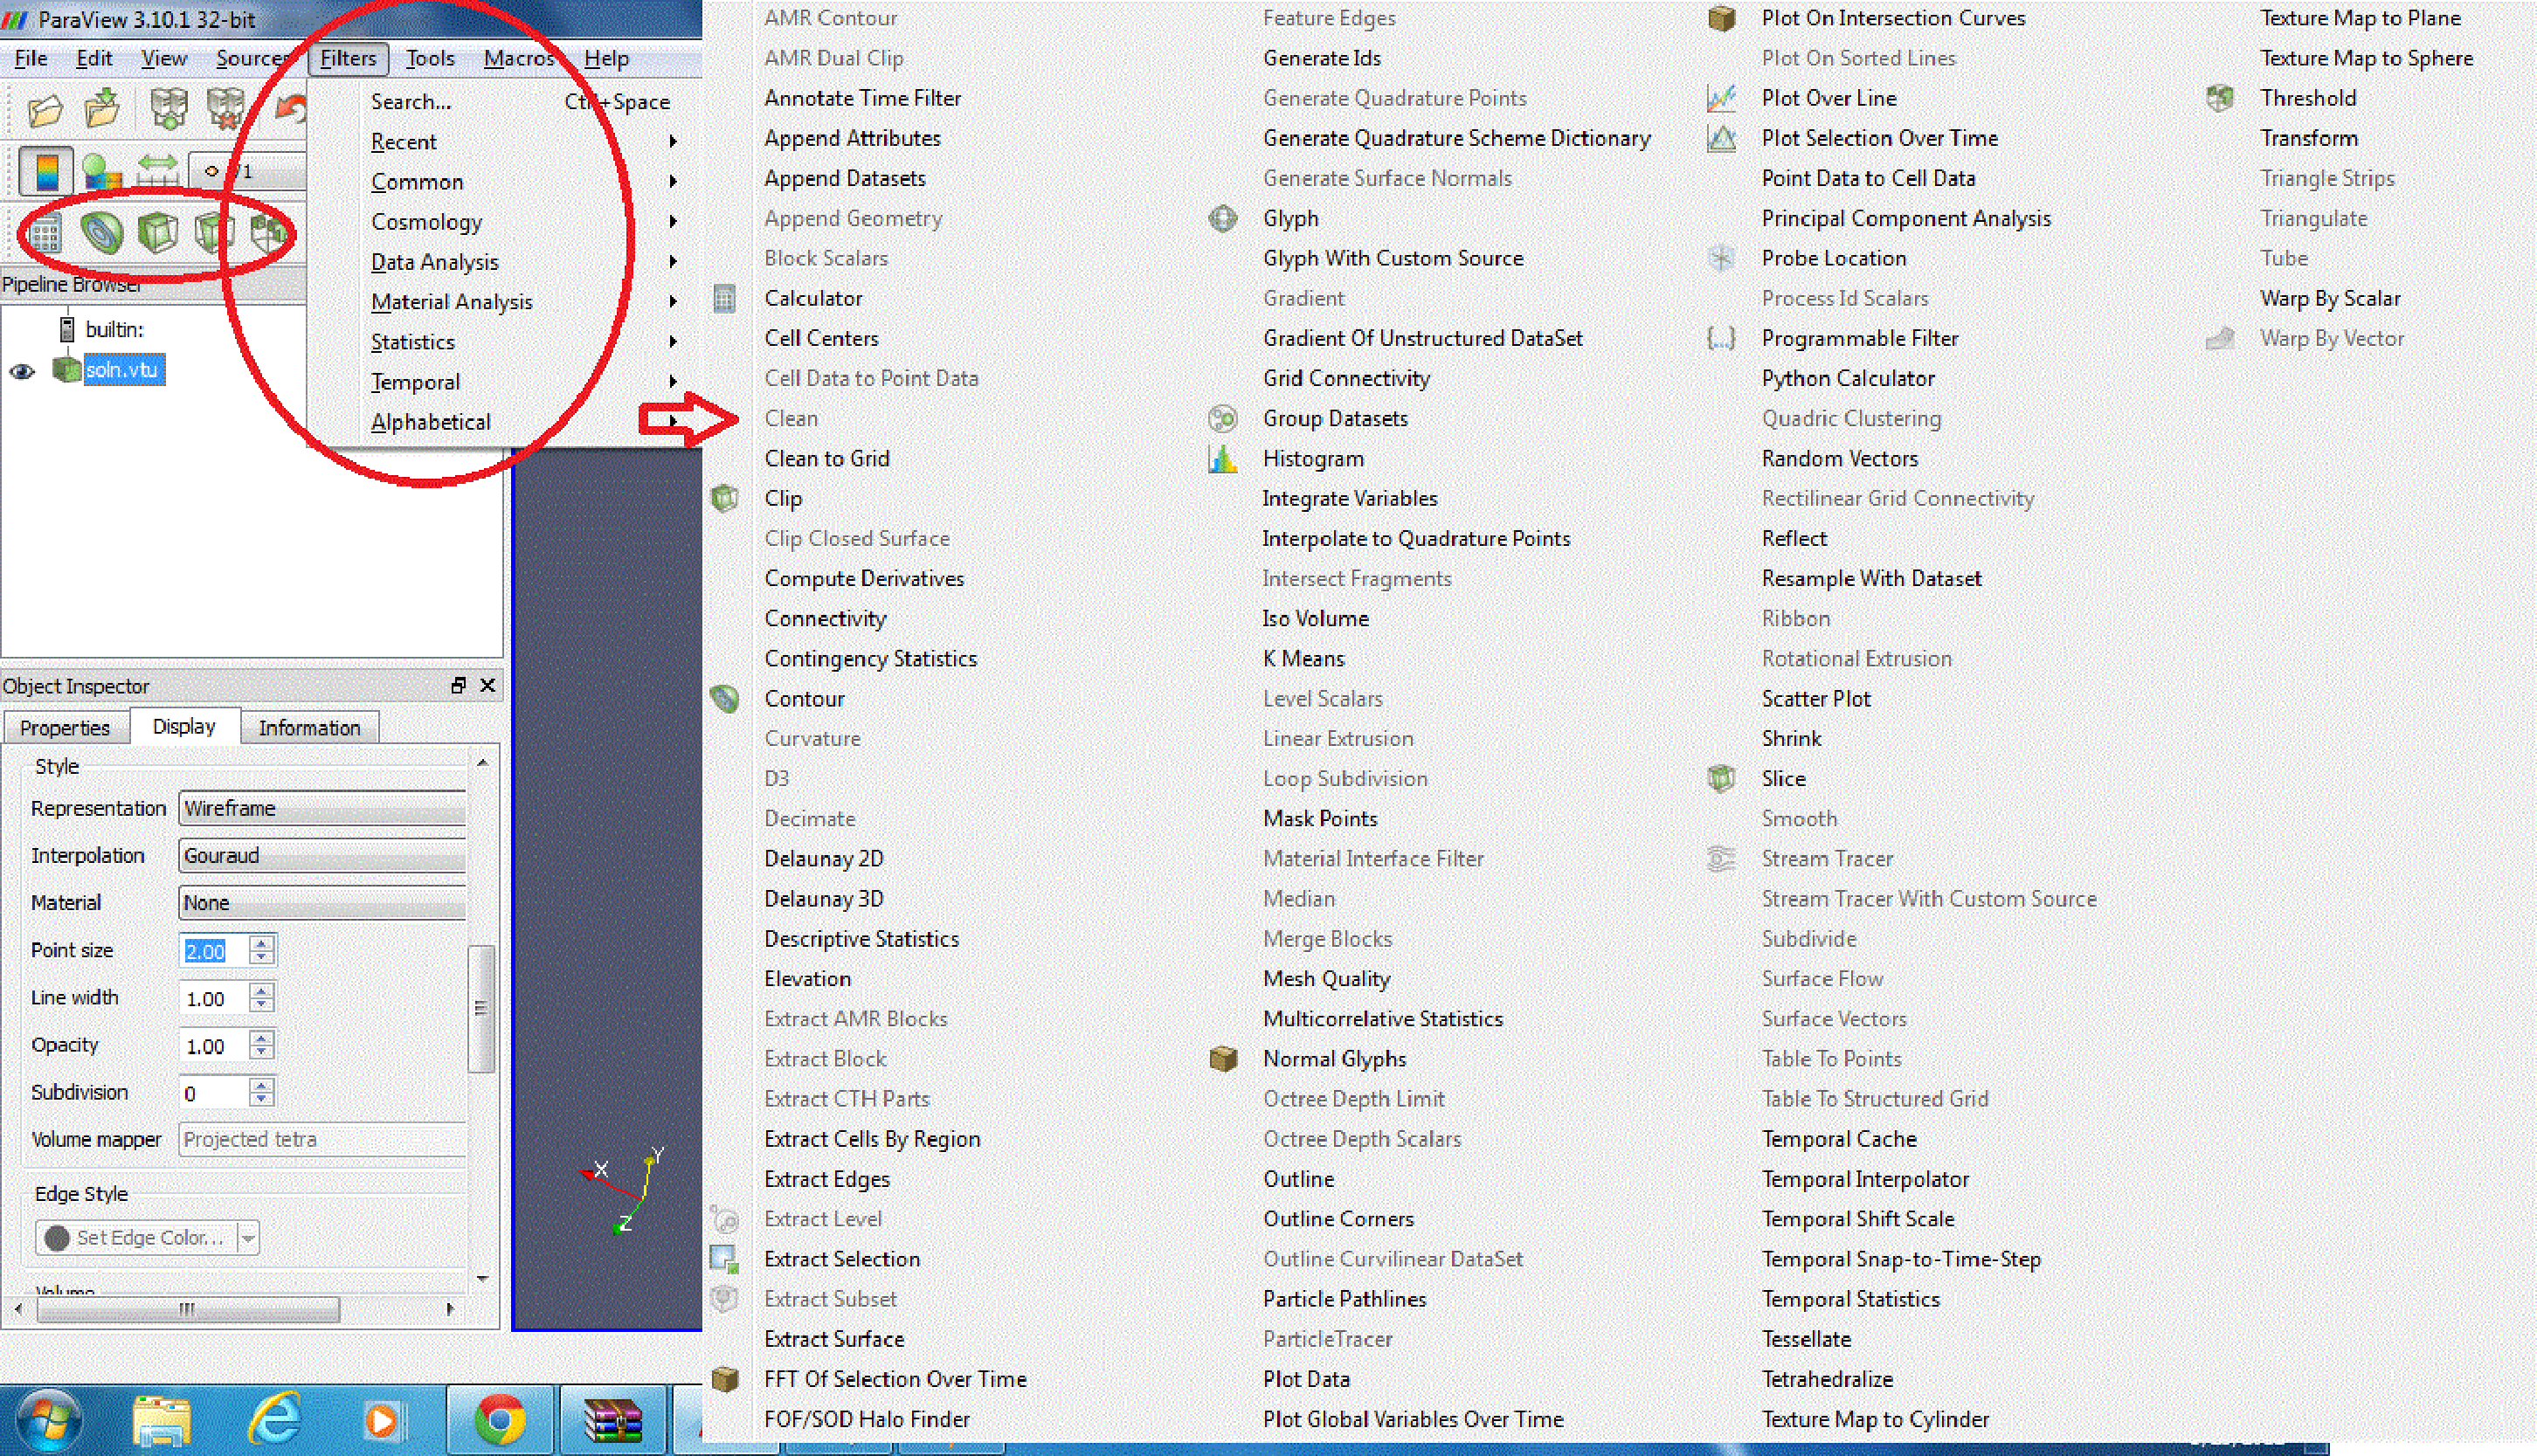
\includegraphics[width=\textwidth]{paraview06}}
\end{DoxyImageNoCaption}


Here are few examples of filters available\+:


\begin{DoxyEnumerate}
\item {\ttfamily Calculator\+:} Evaluates a user-\/defined expression e.\+g $ \frac{1}{2} V1^2 $ and creates a new data array, called here \char`\"{}\+Energy\char`\"{}, containing the result of this expression\+: ~\newline
 
\begin{DoxyImageNoCaption}
  \mbox{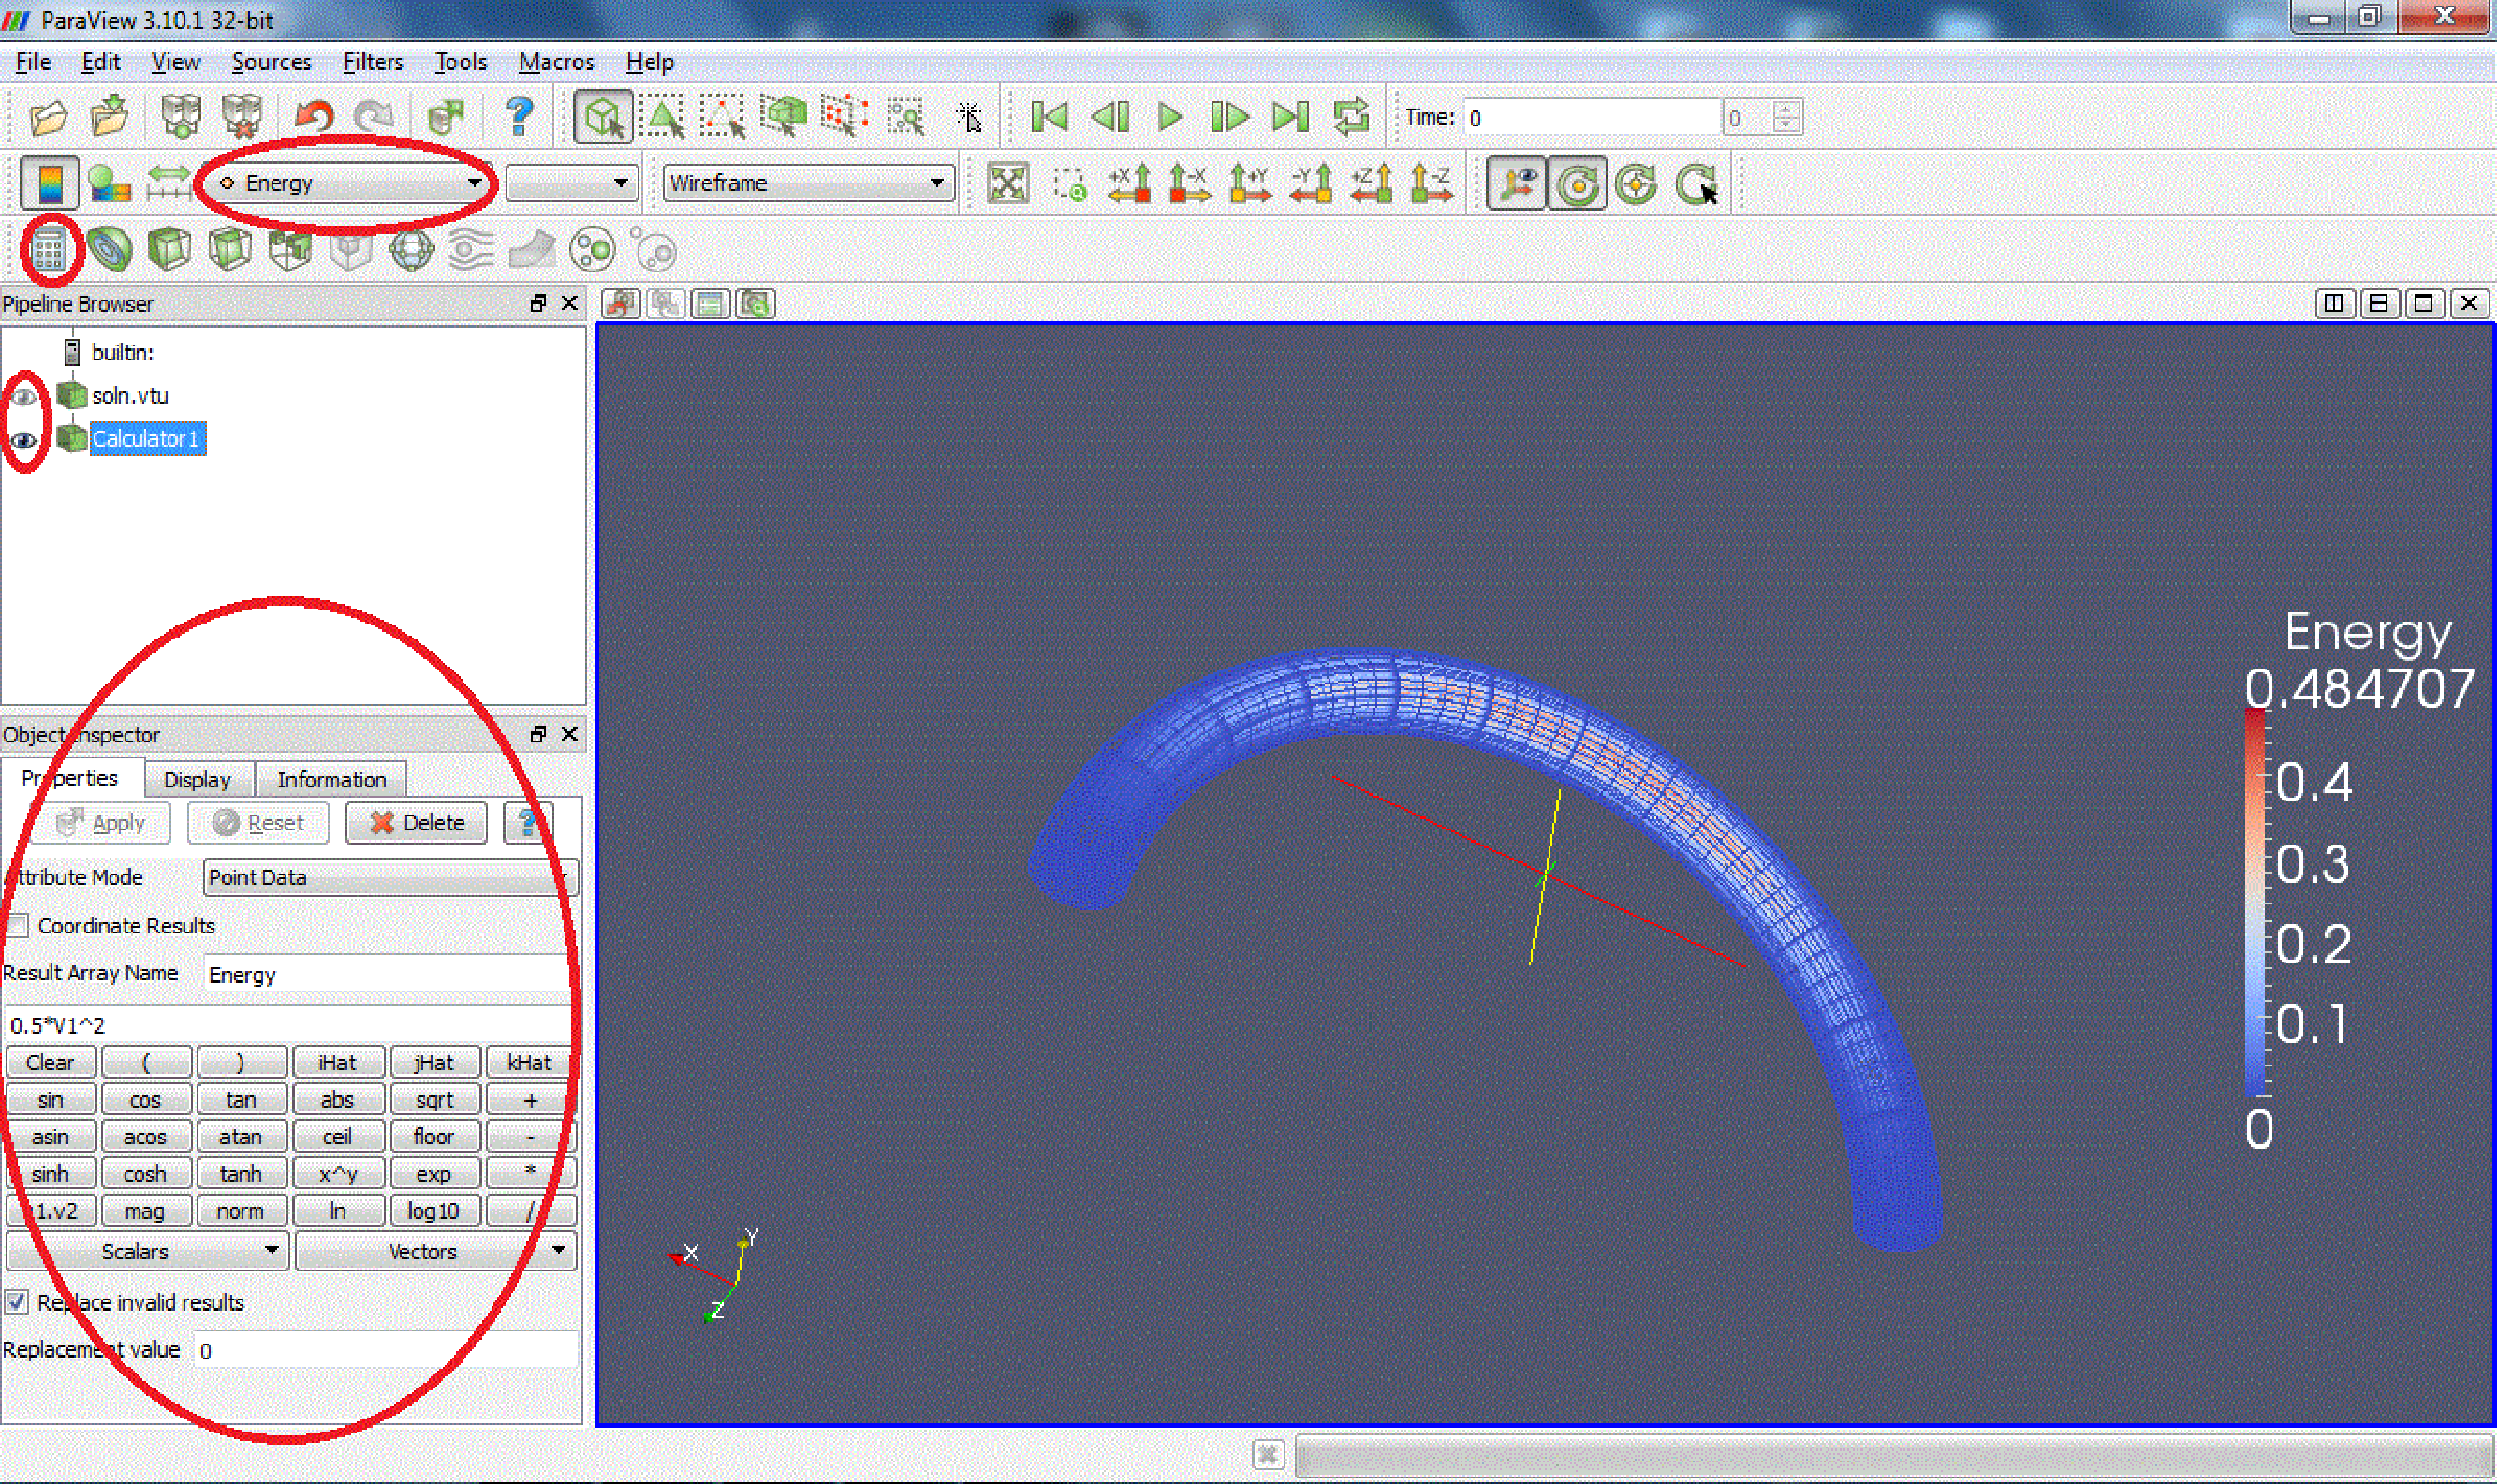
\includegraphics[width=\textwidth]{paraview07}}
\end{DoxyImageNoCaption}
 ~\newline

\item {\ttfamily Contour\+:} Extracts the points, curves or surfaces where a scalar field is equal to a user-\/defined value e.\+g $ V1 = -0.5 $\+: ~\newline
 
\begin{DoxyImageNoCaption}
  \mbox{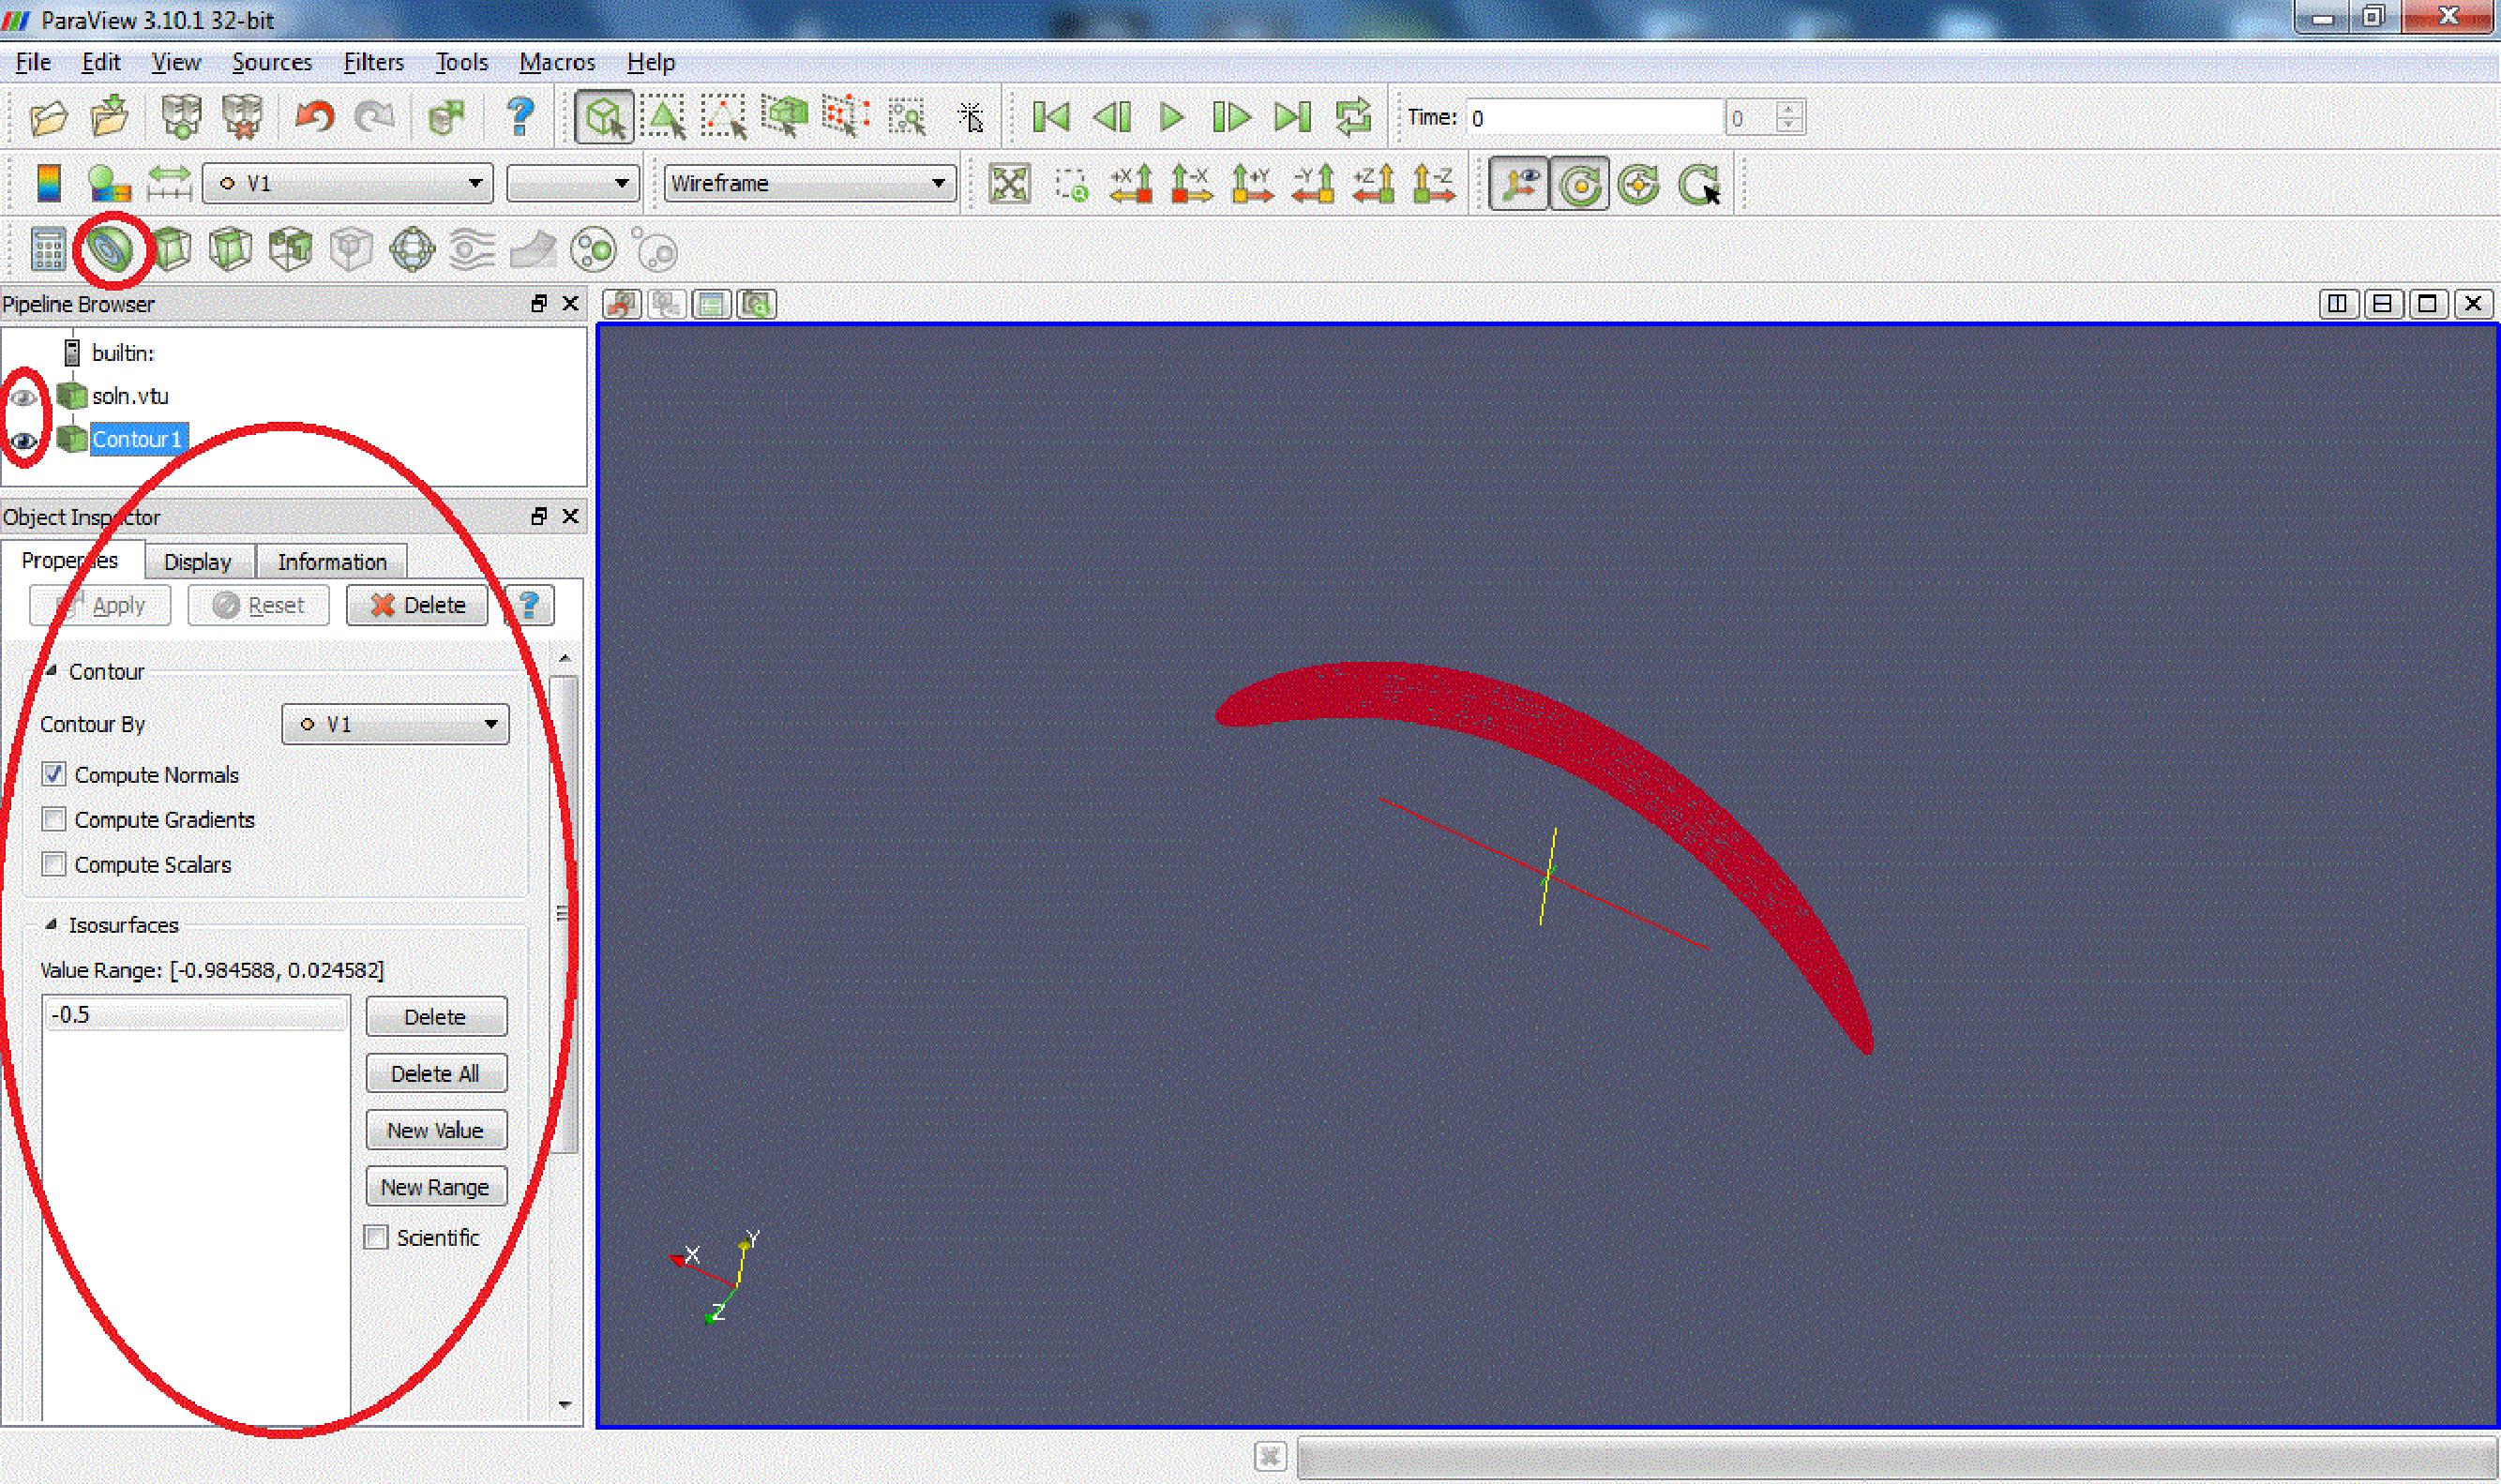
\includegraphics[width=\textwidth]{paraview08}}
\end{DoxyImageNoCaption}
 ~\newline

\item {\ttfamily Clip\+:} Intersects the geometry with a half space. (Warning\+: with some versions of Paraview, zooming on the clipped surface can cause the X server to crash.) ~\newline
 
\begin{DoxyImageNoCaption}
  \mbox{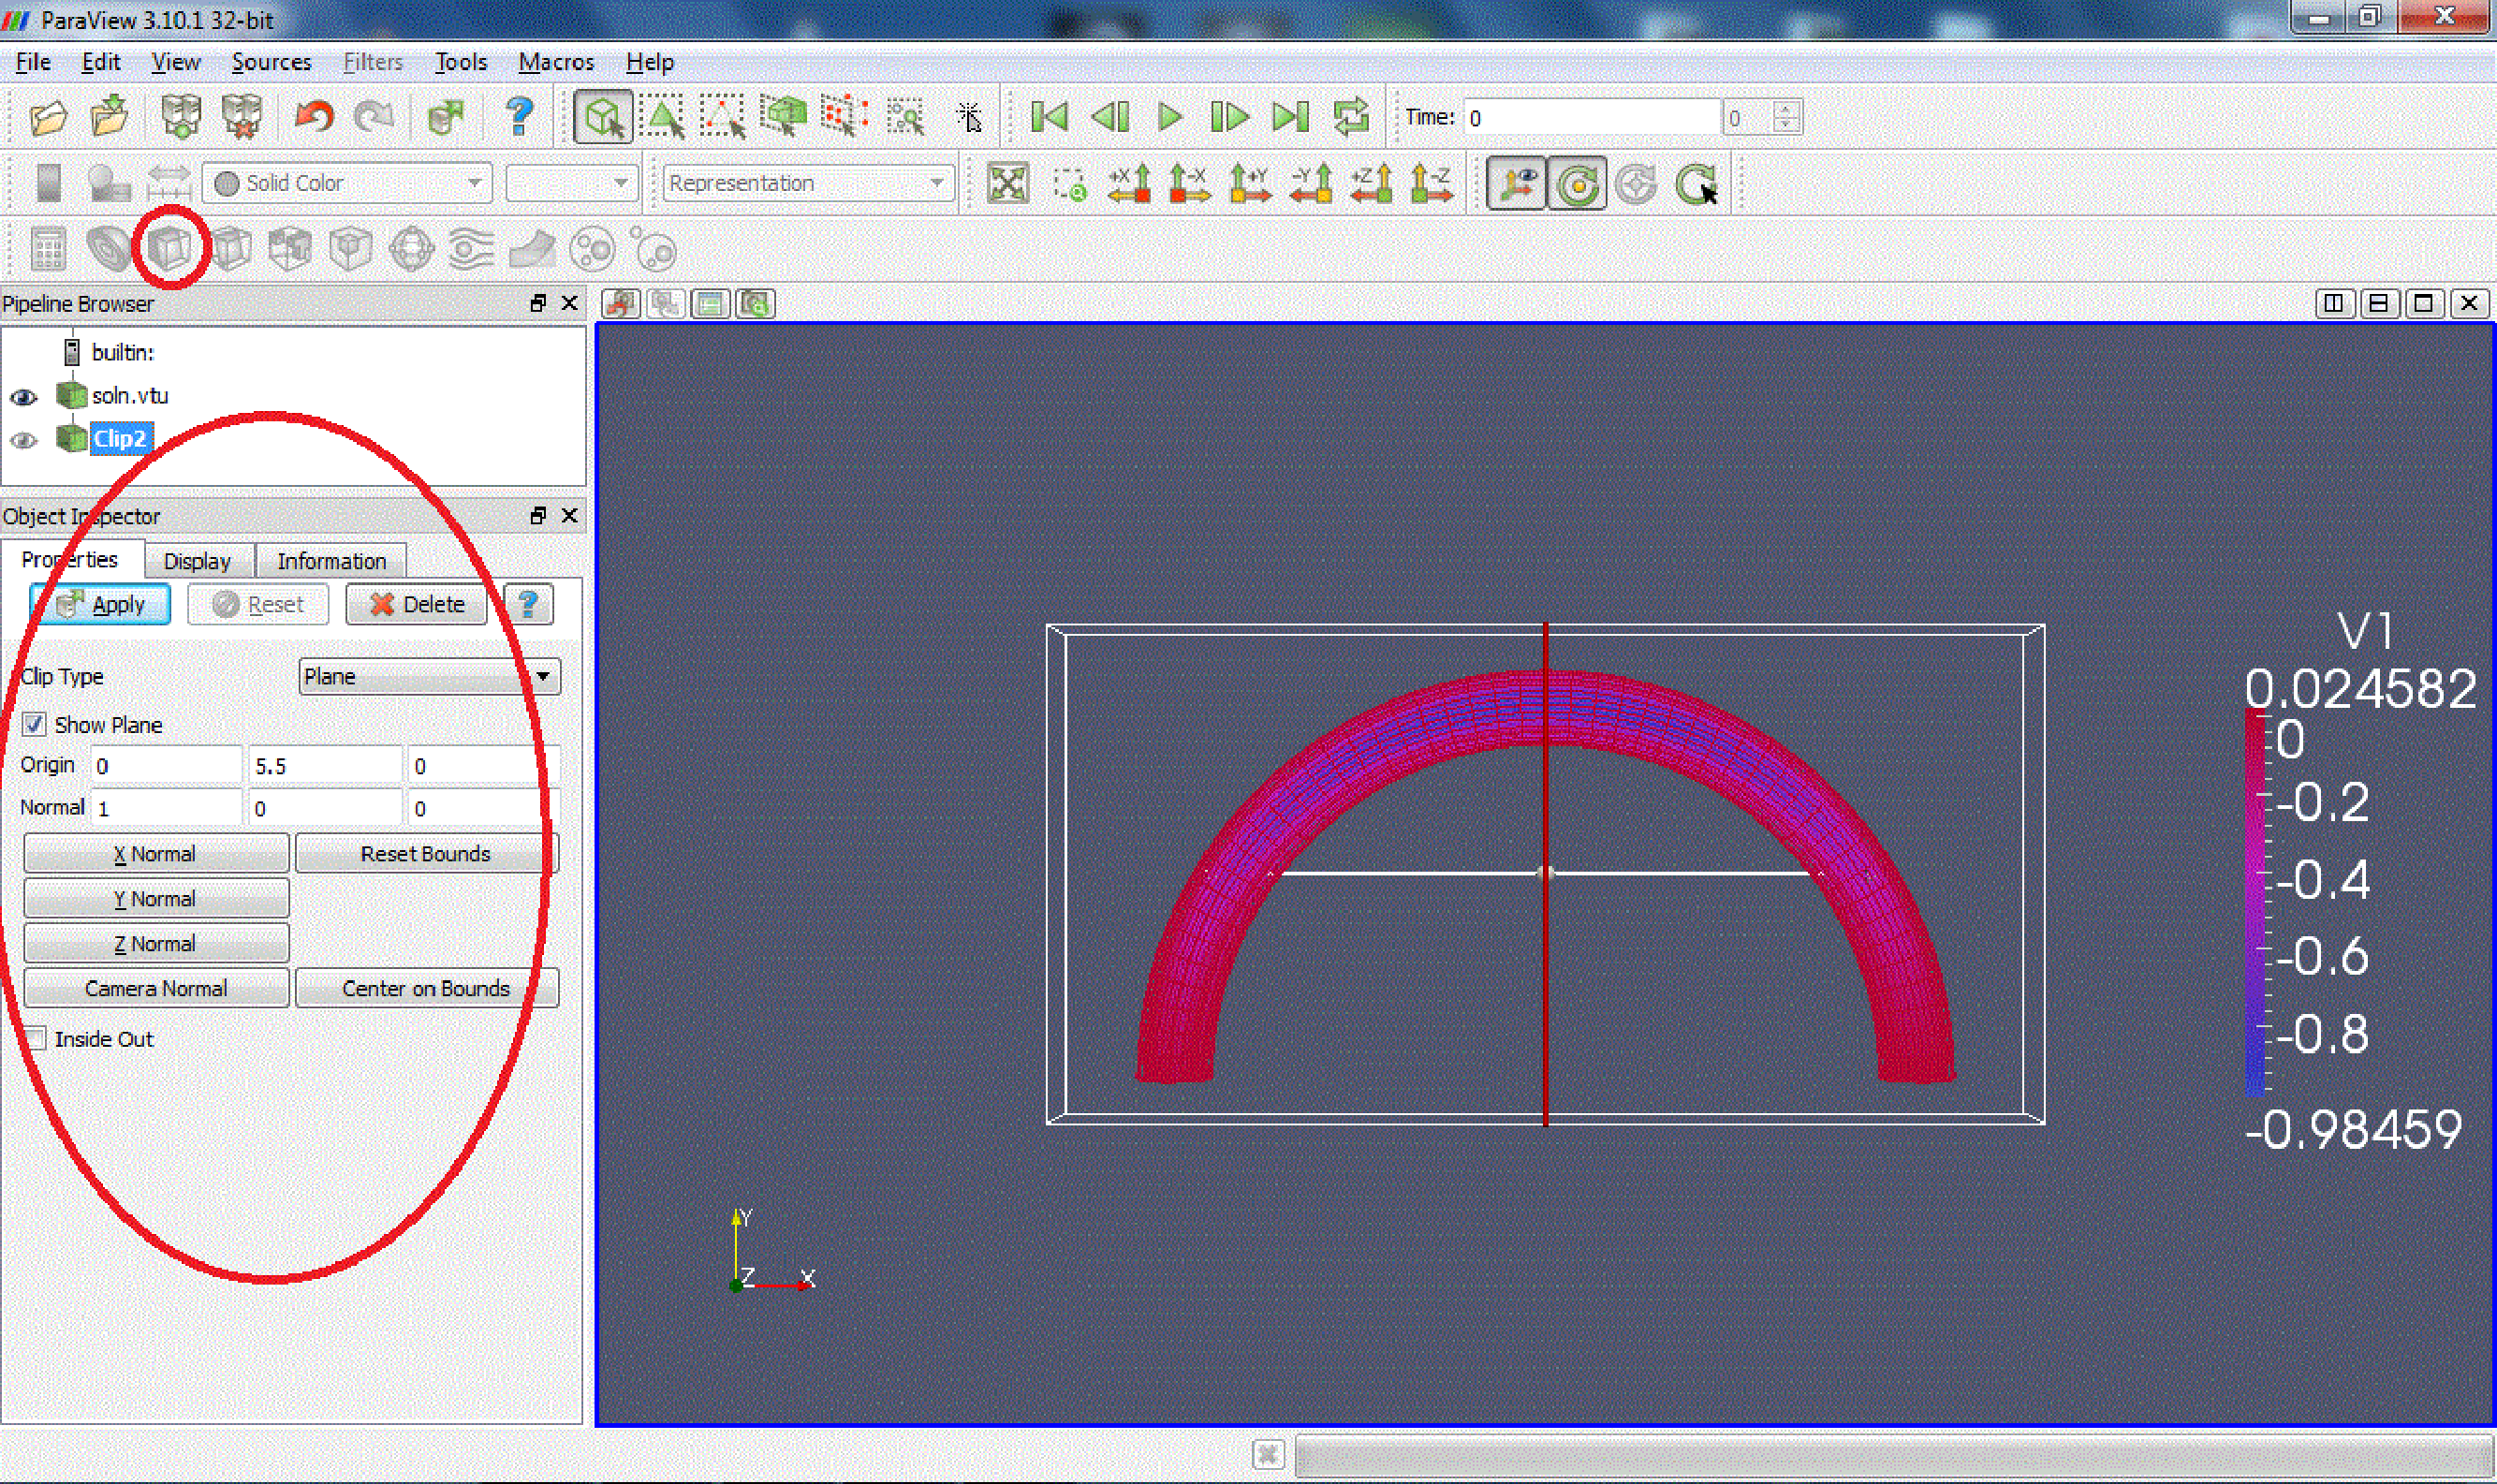
\includegraphics[width=\textwidth]{paraview09}}
\end{DoxyImageNoCaption}
  
\begin{DoxyImageNoCaption}
  \mbox{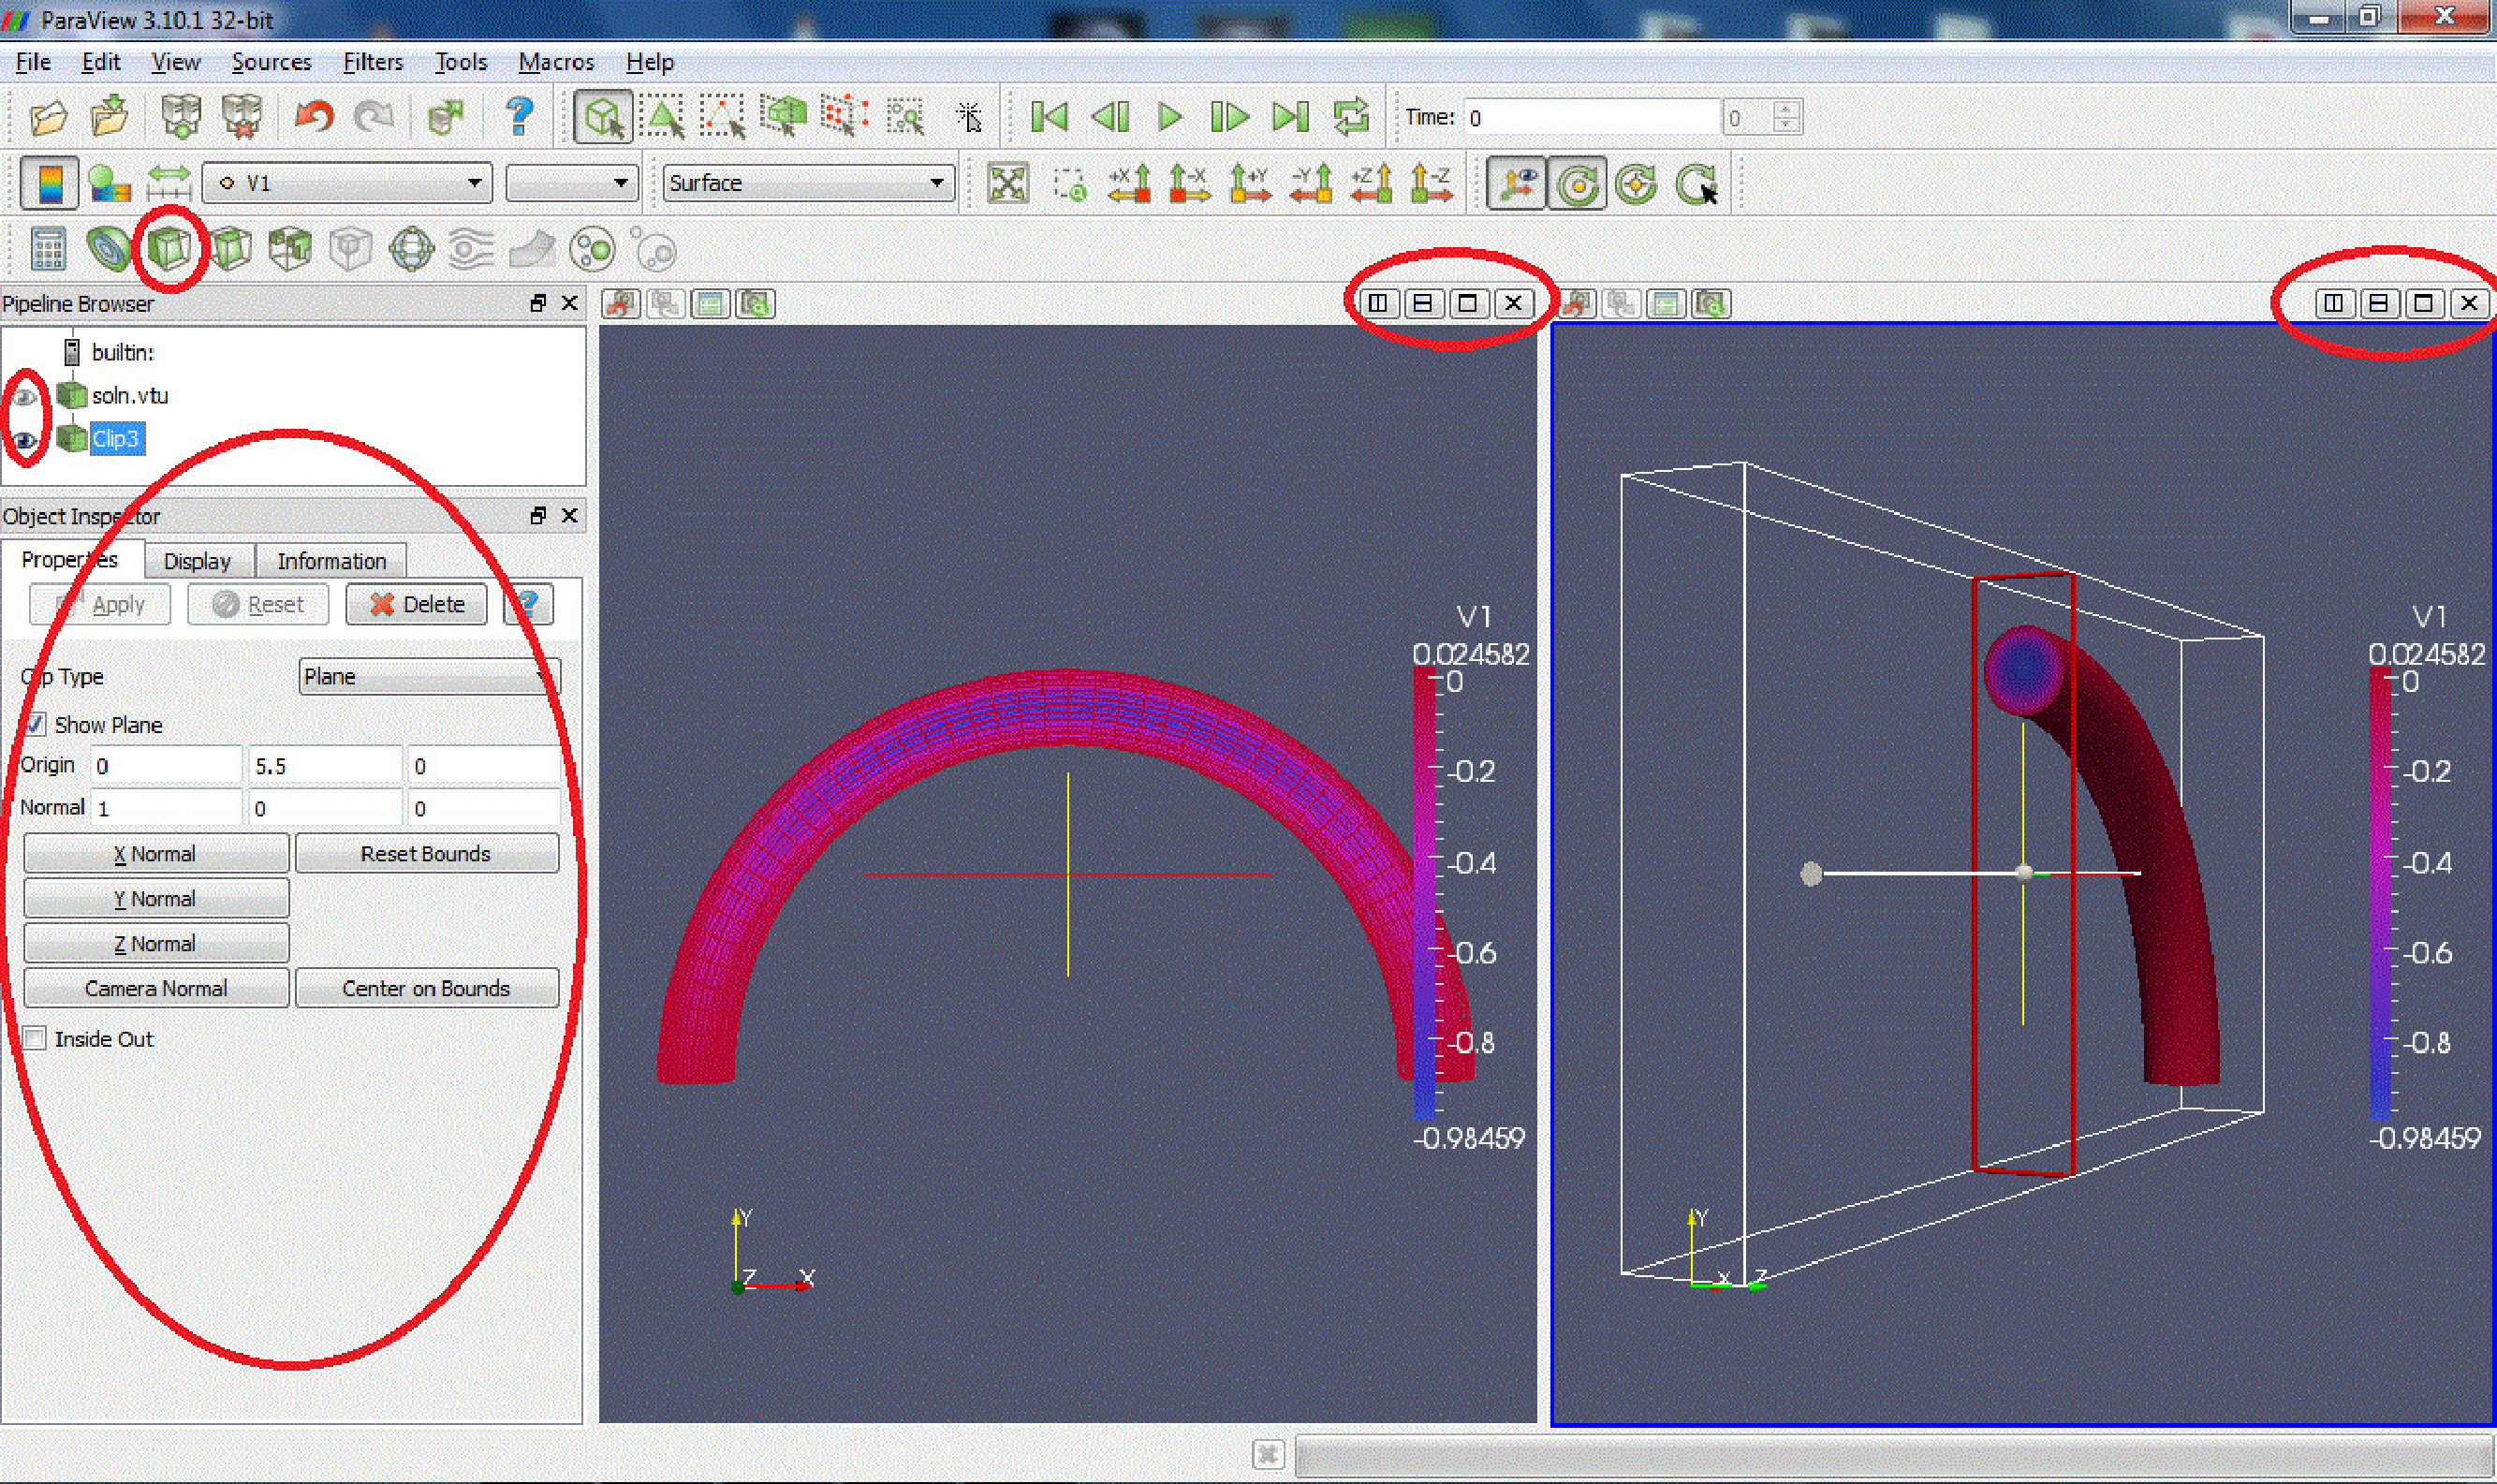
\includegraphics[width=\textwidth]{paraview091}}
\end{DoxyImageNoCaption}
 ~\newline

\item {\ttfamily Slice\+:} Intersects the geometry with a plane. (Warning\+: with some versions of Paraview, zooming on the clipped surface can cause the X server to crash.) ~\newline
 
\begin{DoxyImageNoCaption}
  \mbox{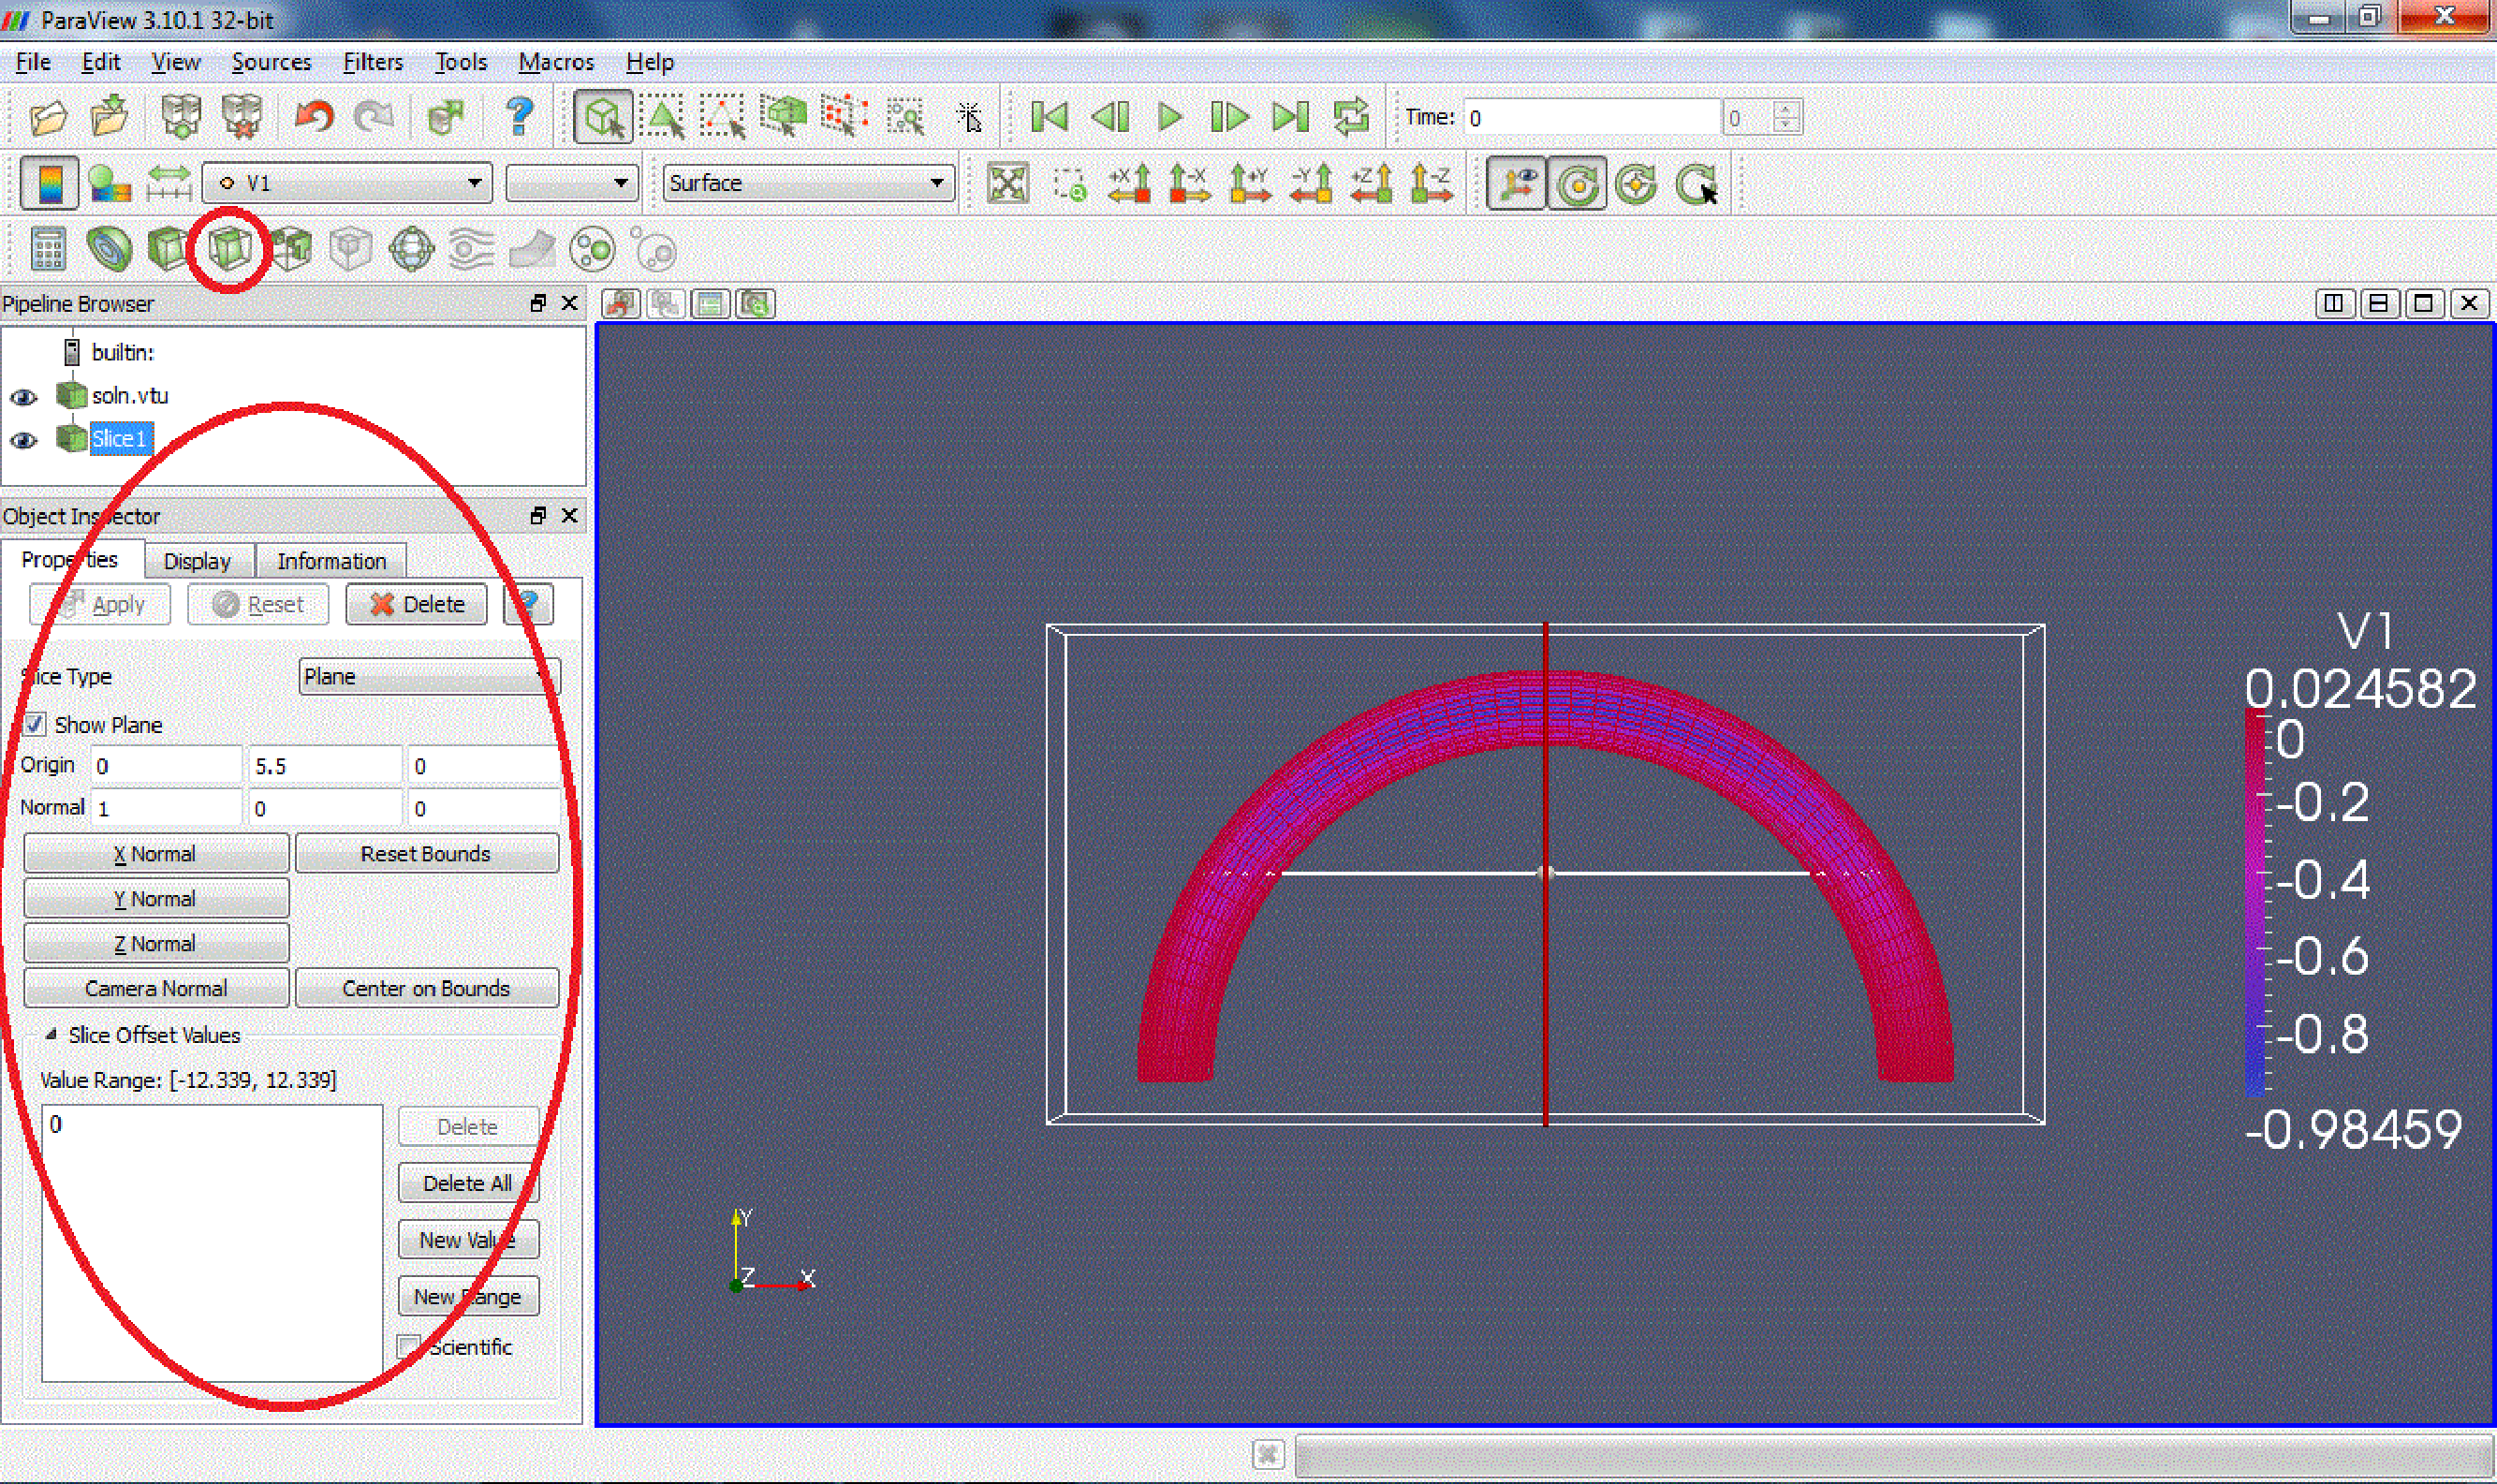
\includegraphics[width=\textwidth]{paraview10}}
\end{DoxyImageNoCaption}
  
\begin{DoxyImageNoCaption}
  \mbox{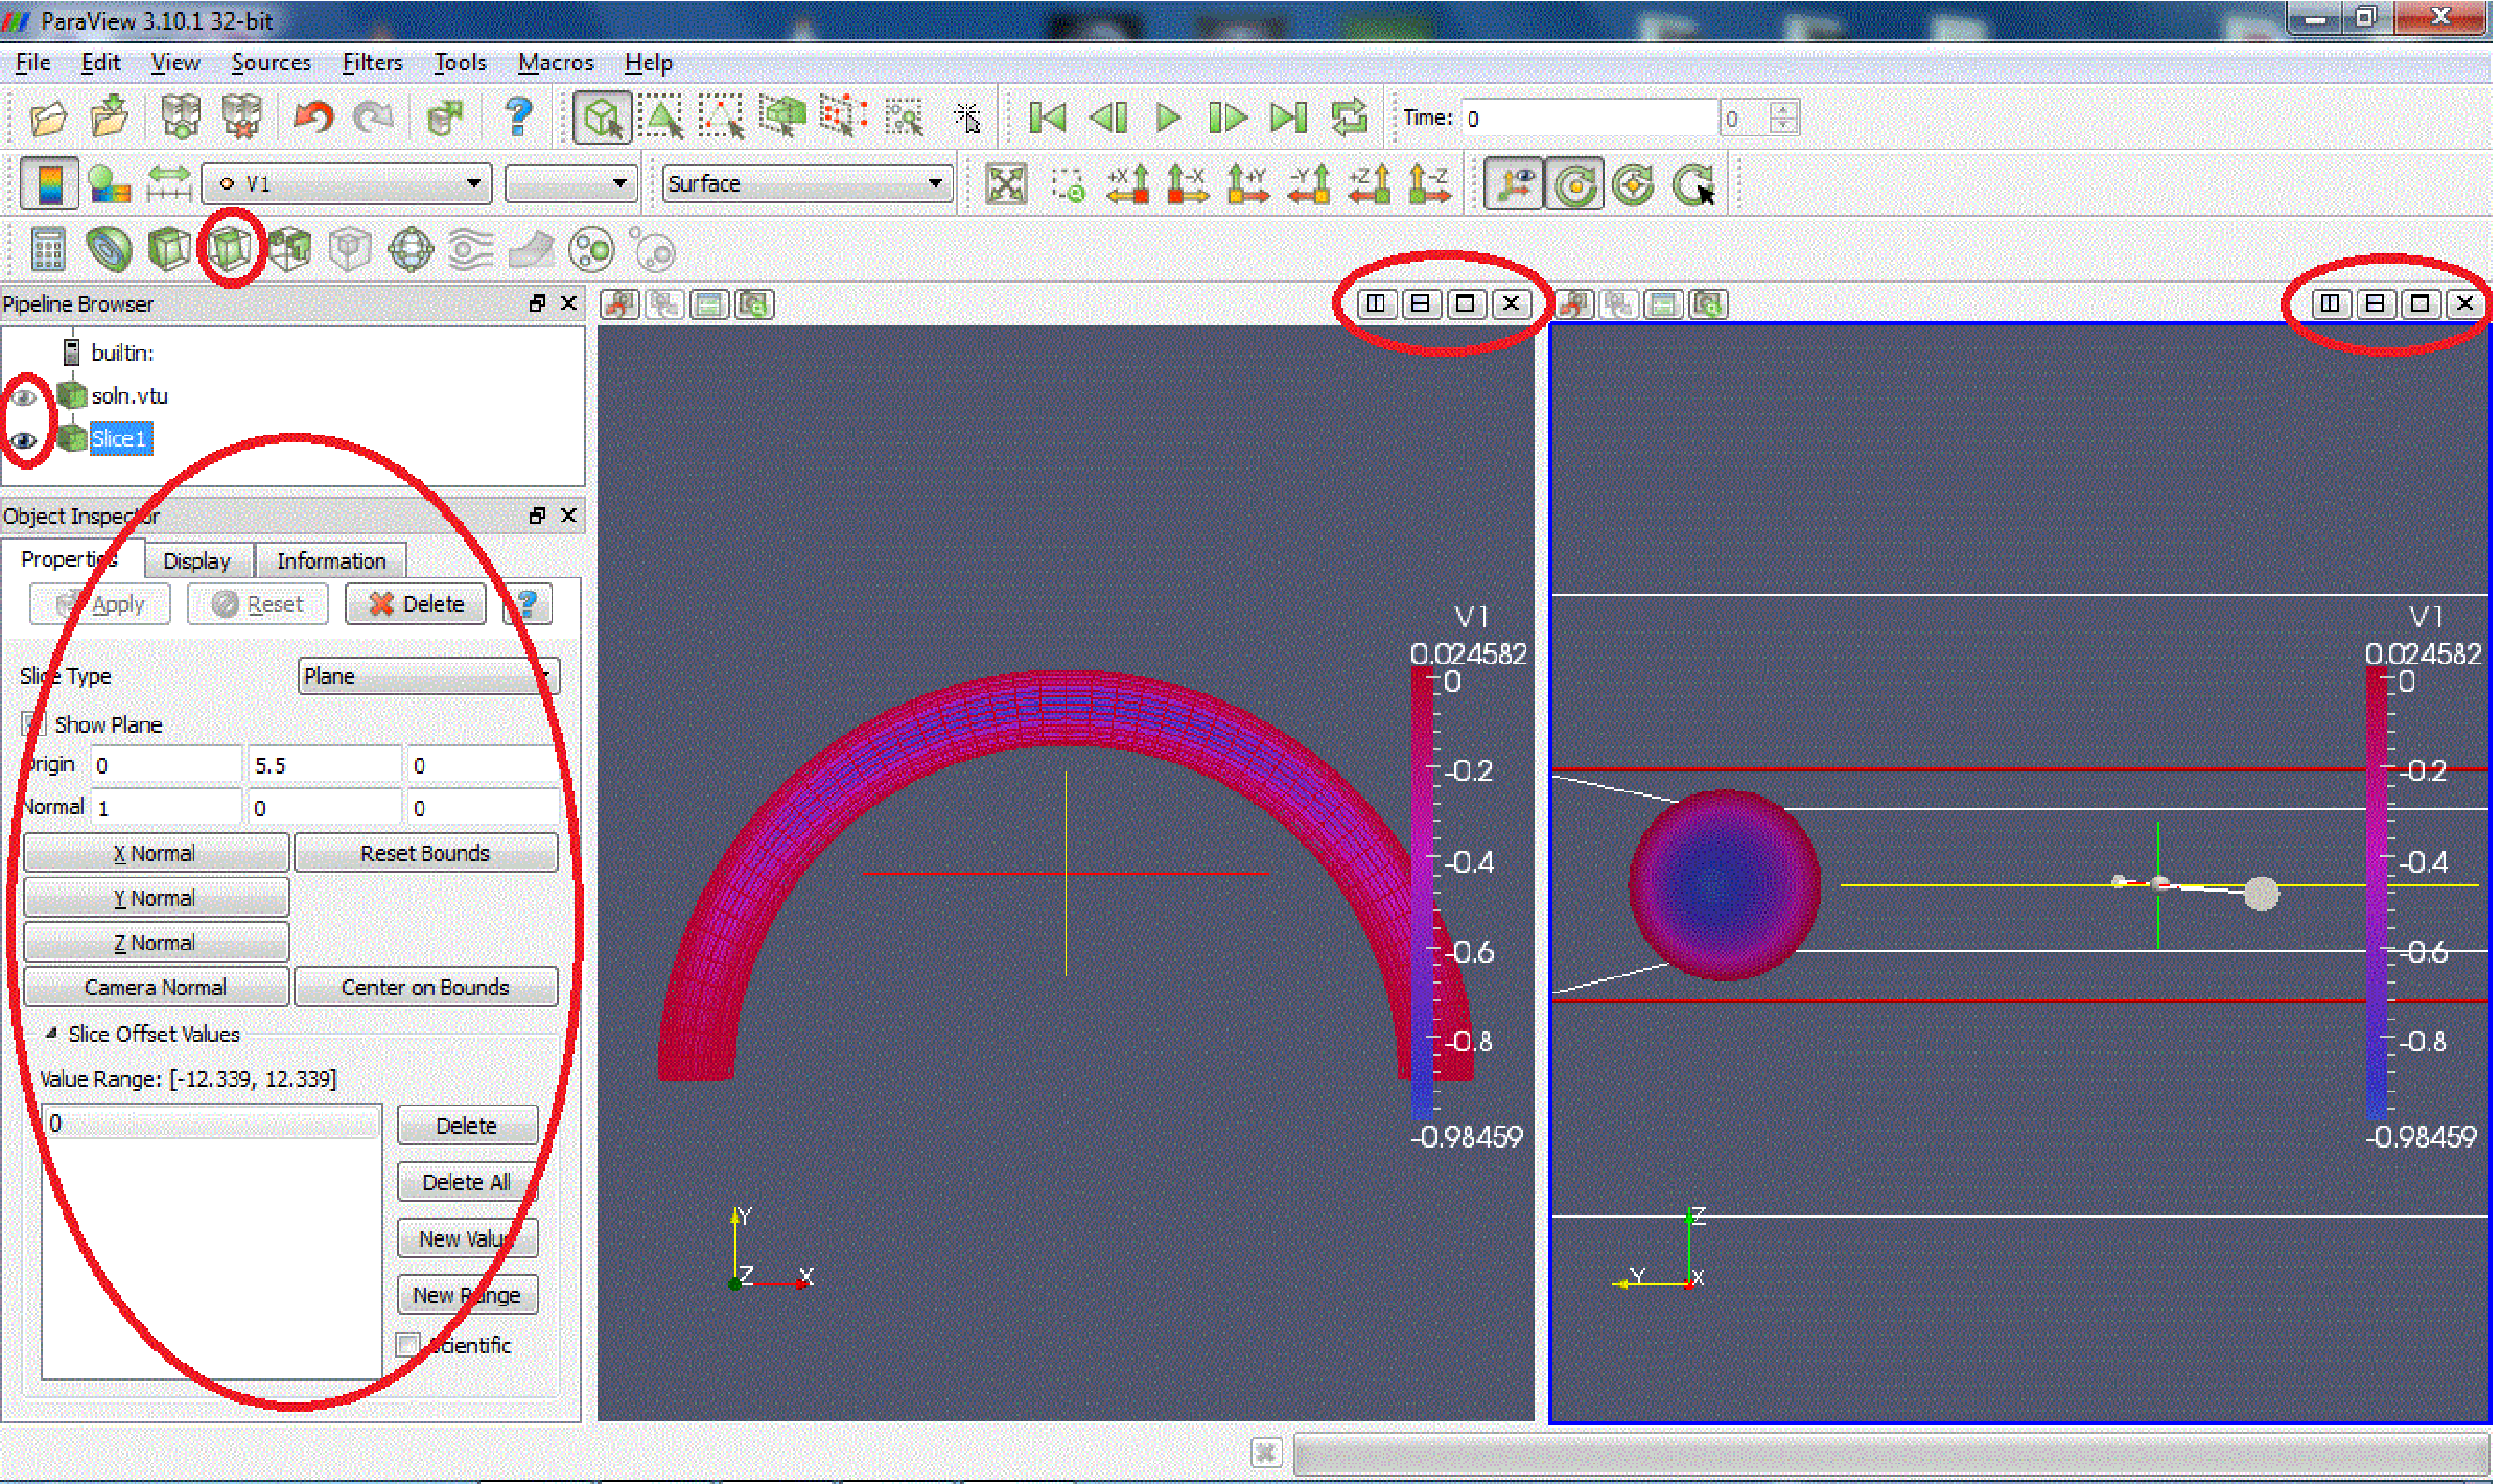
\includegraphics[width=\textwidth]{paraview11}}
\end{DoxyImageNoCaption}
 ~\newline

\item {\ttfamily Threshold\+:} Extracts cells that lie within a specified range of values ~\newline
 
\begin{DoxyImageNoCaption}
  \mbox{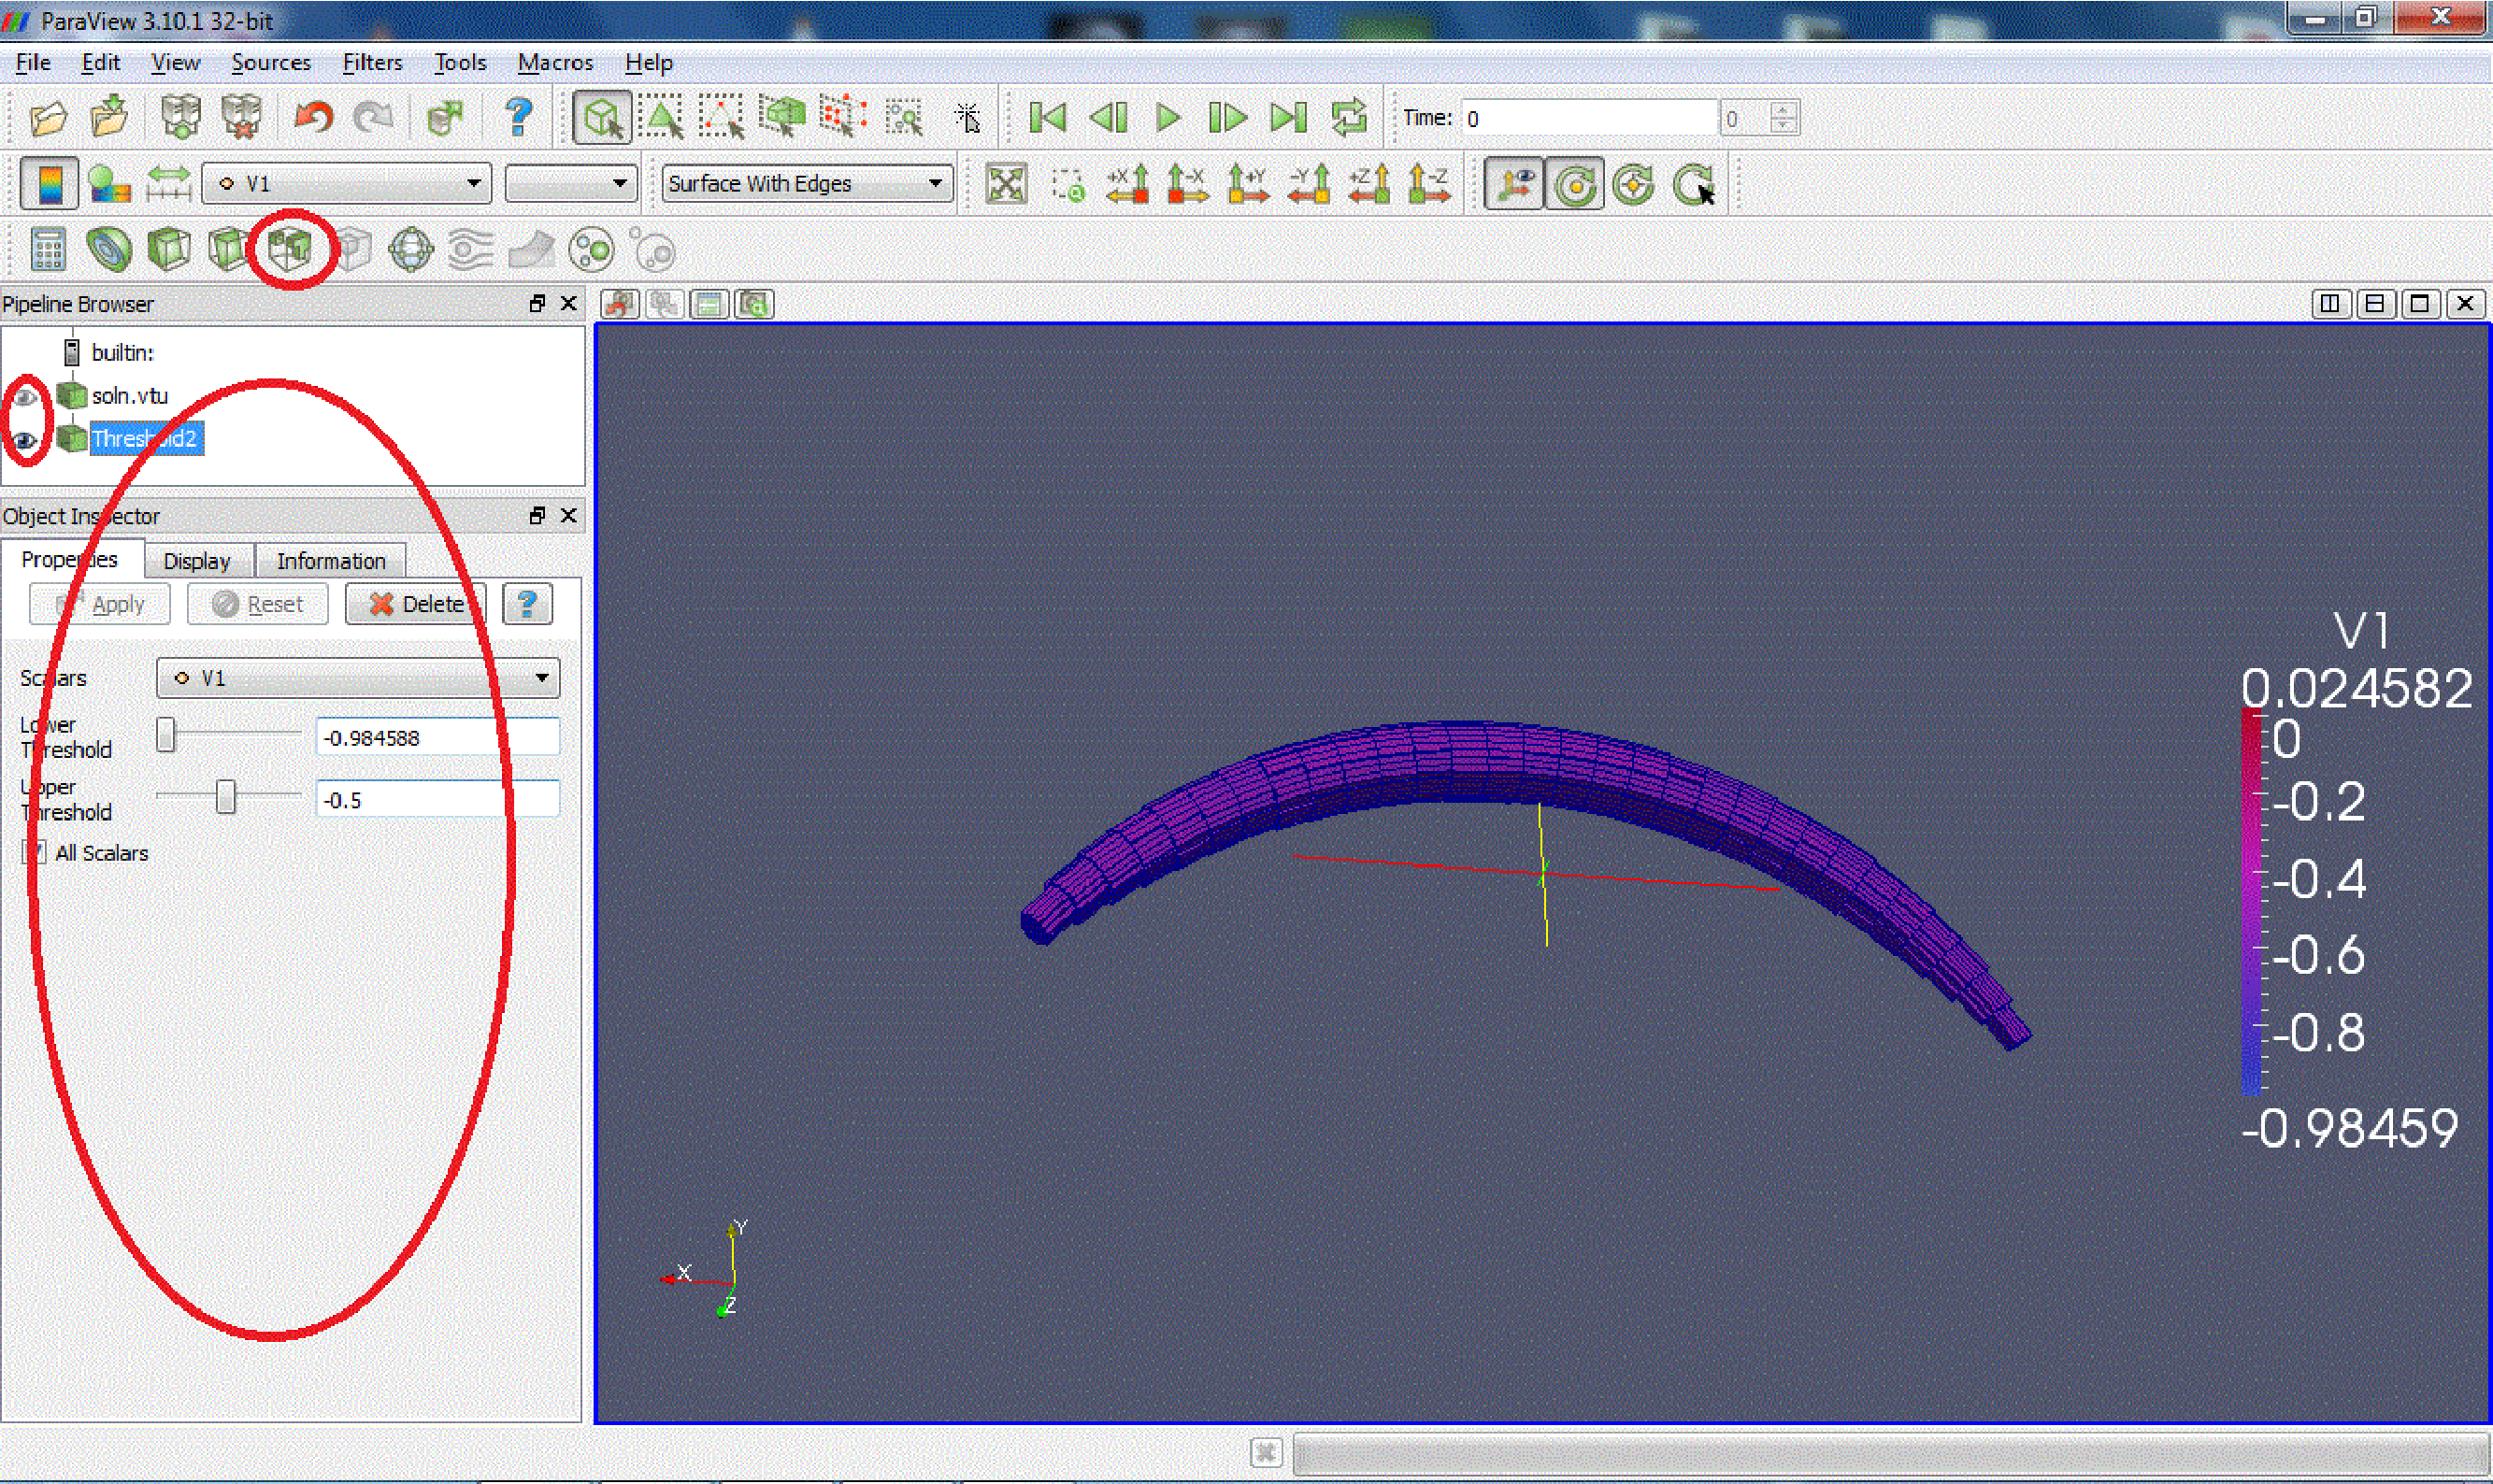
\includegraphics[width=\textwidth]{paraview12}}
\end{DoxyImageNoCaption}

\end{DoxyEnumerate}\hypertarget{index_howto}{}\section{How to ...}\label{index_howto}
\hypertarget{index_outlines}{}\subsection{Select and extract elements}\label{index_outlines}
Click on the button\+: ~\newline
 
\begin{DoxyImageNoCaption}
  \mbox{
\includegraphics[width=0.03\textwidth]{selec_button}}
\end{DoxyImageNoCaption}
 {\ttfamily Select} {\ttfamily Cells} {\ttfamily On} to select elements on the surface (2D selection) ~\newline
 
\begin{DoxyImageNoCaption}
  \mbox{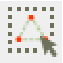
\includegraphics[width=0.03\textwidth]{selec2_button}}
\end{DoxyImageNoCaption}
 {\ttfamily Select} {\ttfamily Points} {\ttfamily On} to select points on the surface (2D selection) ~\newline
 
\begin{DoxyImageNoCaption}
  \mbox{
\includegraphics[width=0.03\textwidth]{selec3_button}}
\end{DoxyImageNoCaption}
 {\ttfamily Select} {\ttfamily Cells} {\ttfamily Through} to select elements through the region selected (3D selection) ~\newline
 
\begin{DoxyImageNoCaption}
  \mbox{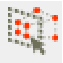
\includegraphics[width=0.03\textwidth]{selec4_button}}
\end{DoxyImageNoCaption}
 {\ttfamily Select} {\ttfamily Points} {\ttfamily Through} to select points through the region selected (3D selection) ~\newline
When your selection is highlighted, go to {\ttfamily Filters-\/$>$Data} {\ttfamily Analysis-\/$>$Extract} {\ttfamily Selection} and  
\begin{DoxyImageNoCaption}
  \mbox{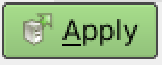
\includegraphics[width=0.07\textwidth]{apply_button}}
\end{DoxyImageNoCaption}
 {\ttfamily Apply} the filter to extract the selected elements. You can now modify or apply filters on the extracted data only.

Here is an example of extraction of the surface elements of the curved pipe data\+:

 
\begin{DoxyImageNoCaption}
  \mbox{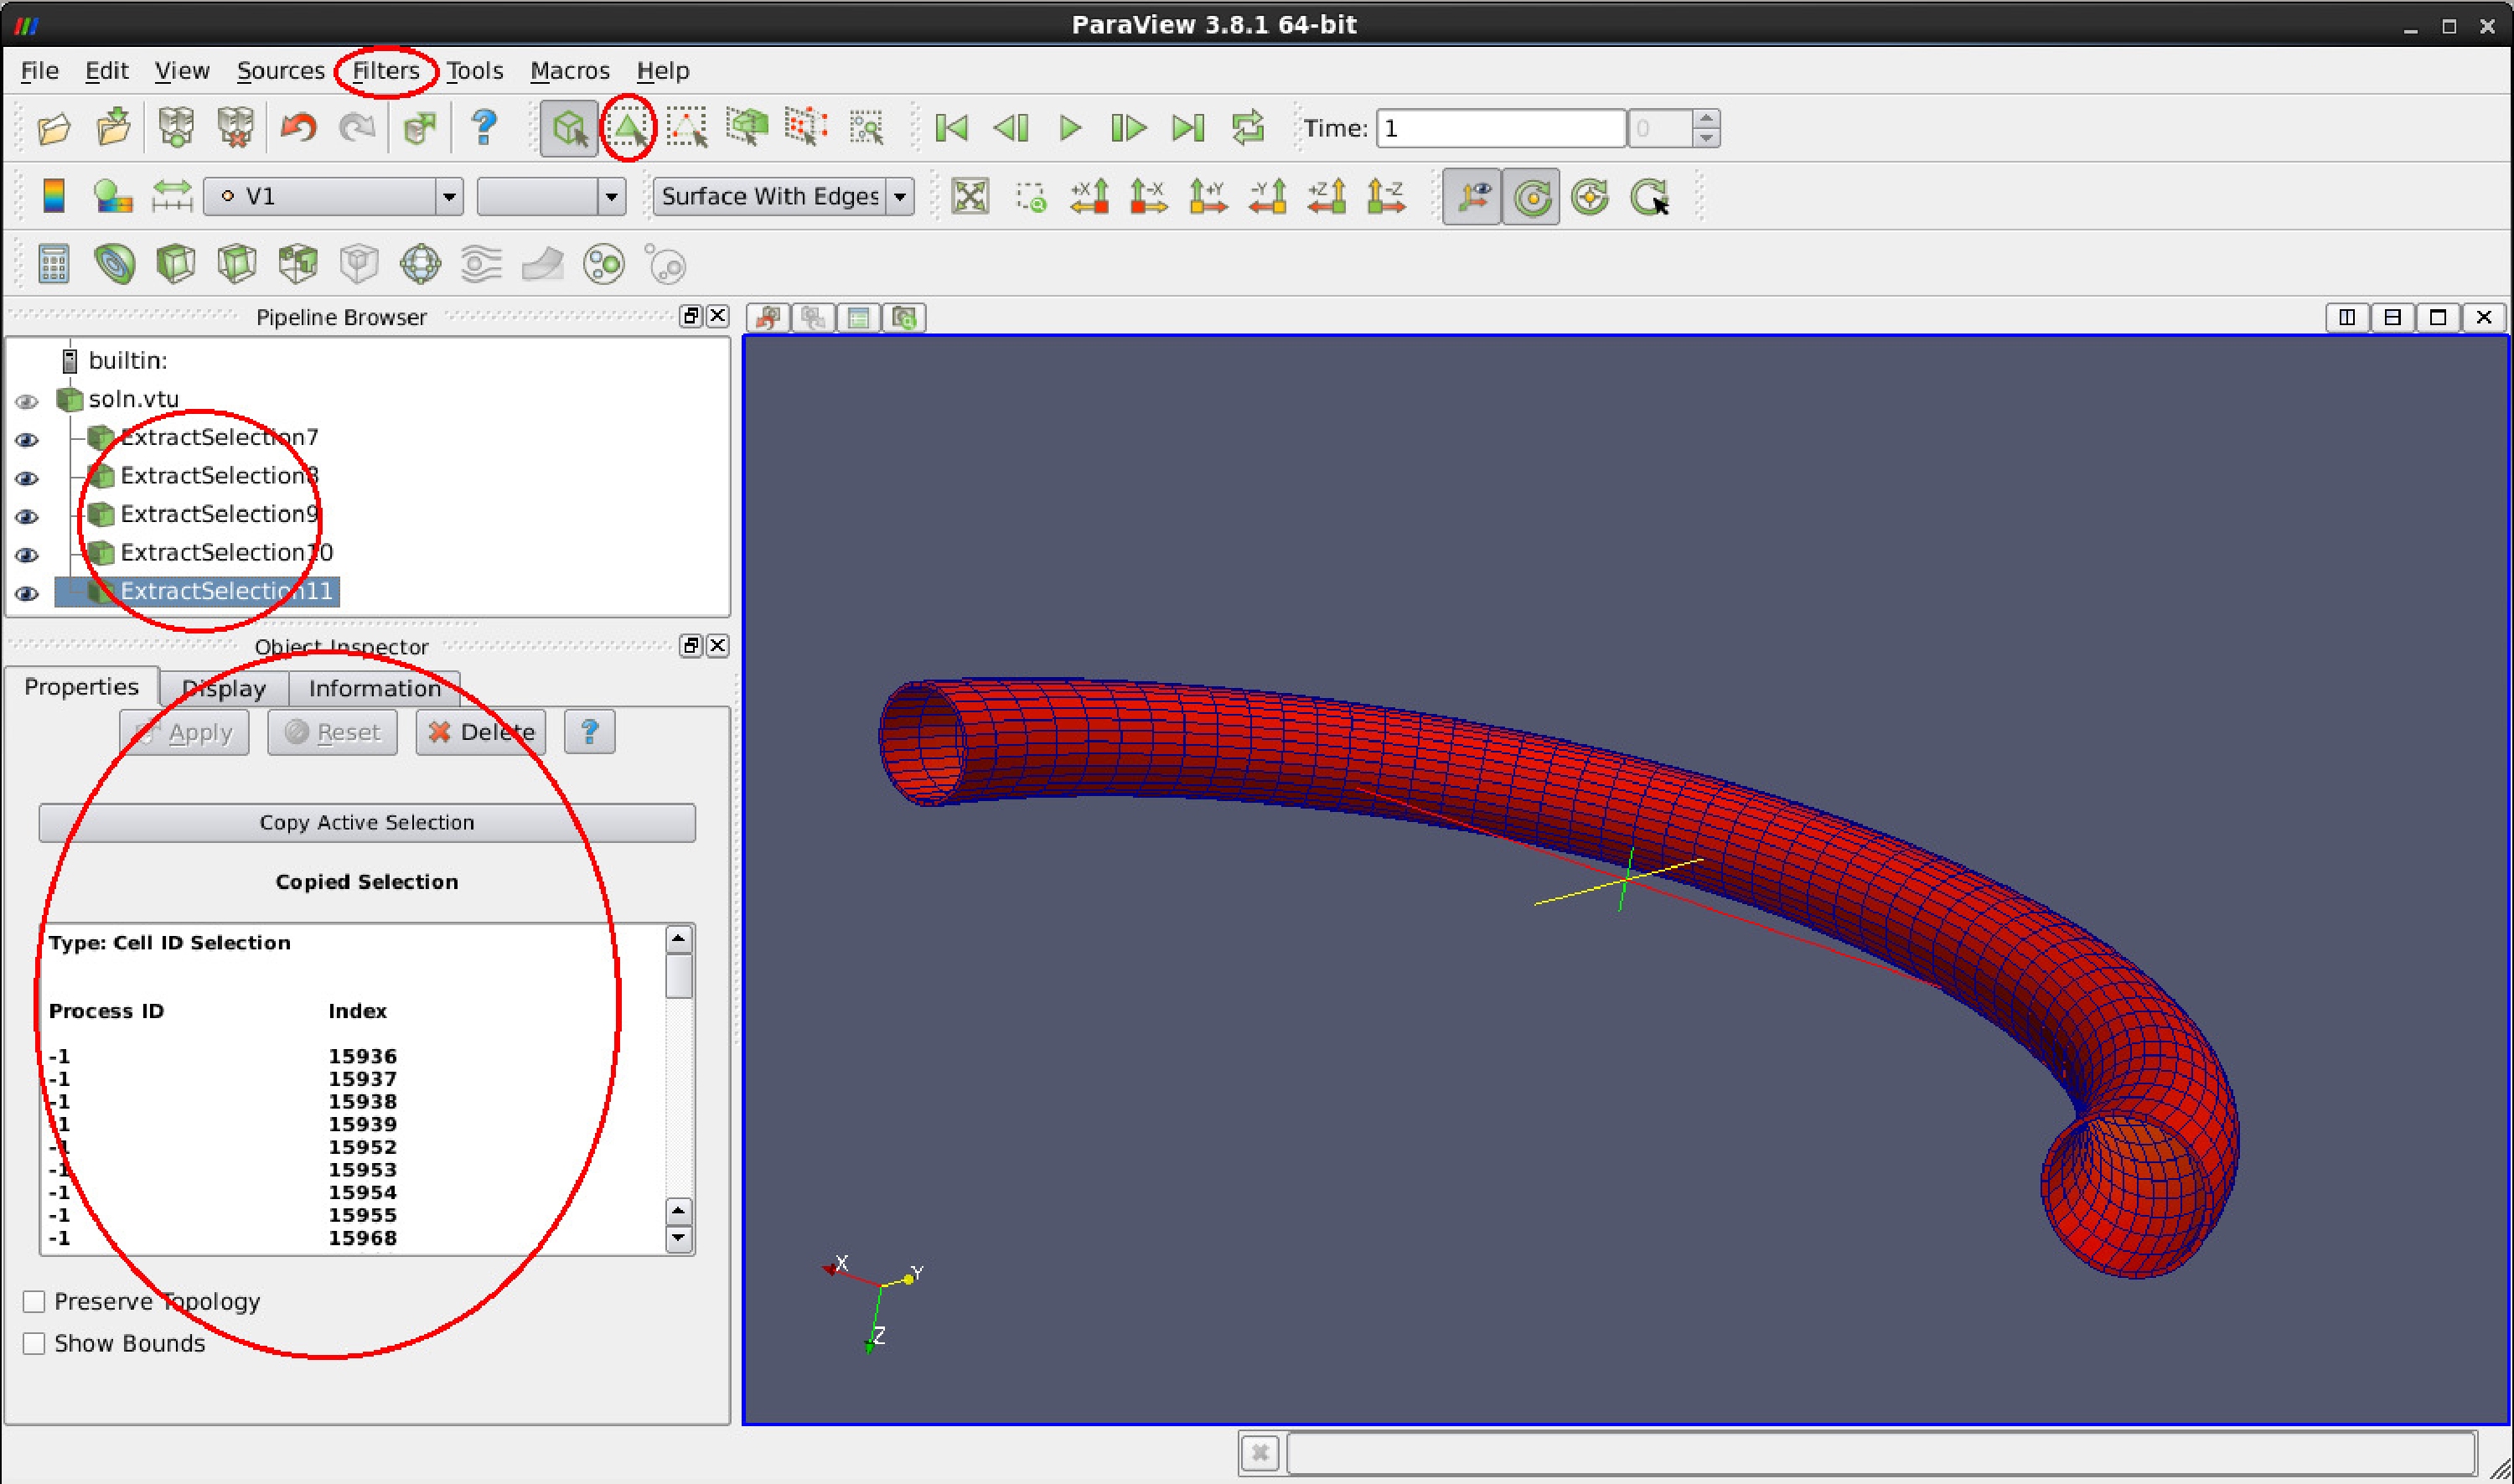
\includegraphics[width=\textwidth]{how_to_01}}
\end{DoxyImageNoCaption}




 

 \hypertarget{index_pdf}{}\section{P\+D\+F file}\label{index_pdf}
A \href{../latex/refman.pdf}{\tt pdf version} of this document is available. \end{document}
